% ==========================================================================
%  Screening on the Wrong Null:
%  When a No-Content Hypothesis Does Not Imply a Zero Statistic
%
%  Finance only.  The machine learning half of the earlier draft is parked on
%  a separate branch; nothing was deleted from the repository, only from this
%  document.
%
%  Every number in this file comes from tables/macros.tex, from
%  tables/macros_alpha.tex, or from an \input{} of a generated table.  Nothing
%  is typed by hand.  If a number here does not have a macro behind it, that
%  is a bug.
% ==========================================================================

\documentclass{article}

% Named preprint build: [preprint] shows the author block and drops the line
% numbers.  The repository URL in the abstract is the real one and the
% repository is public, so the build is internally consistent as it stands.
% For a double-blind submission switch to plain \usepackage{neurips_2023} and
% replace the URL with an anonymised mirror, in the same commit, or the author
% is recoverable from the link.
\usepackage[preprint]{neurips_2023}

\usepackage[utf8]{inputenc}
\usepackage[T1]{fontenc}
\usepackage{hyperref}
\usepackage{url}
\usepackage{booktabs}
\usepackage{amsfonts}
\usepackage{amsmath}
\usepackage{nicefrac}
\usepackage{microtype}
\usepackage{graphicx}
% Generated tables are wrapped in an adjustbox with max width=\linewidth,
% so a wide one shrinks to the text block instead of into the margin.
\usepackage{adjustbox}
\usepackage{xspace}
\usepackage{natbib}

% generated by bzoo.report.tables on 2026-08-01
% do not edit by hand; every number in the paper text comes from here
\newcommand{\bzoonullMeanSdEw}{0.889\xspace}
\newcommand{\bzoonullMeanKurtEw}{2.81\xspace}
\newcommand{\bzoonullMeanExceedEwPct}{3.0\xspace}
\newcommand{\bzoonullMeanThreeEwPct}{$5.2\times 10^{-3}$\xspace}
\newcommand{\bzoonullFfSdEw}{1.150\xspace}
\newcommand{\bzoonullFfKurtEw}{2.97\xspace}
\newcommand{\bzoonullFfExceedEwPct}{9.2\xspace}
\newcommand{\bzoonullFfThreeEwPct}{0.8\xspace}
\newcommand{\bzoonullMeanSdVw}{1.026\xspace}
\newcommand{\bzoonullMeanKurtVw}{3.11\xspace}
\newcommand{\bzoonullMeanExceedVwPct}{6.3\xspace}
\newcommand{\bzoonullMeanThreeVwPct}{0.5\xspace}
\newcommand{\bzoonullFfSdVw}{1.405\xspace}
\newcommand{\bzoonullFfKurtVw}{3.30\xspace}
\newcommand{\bzoonullFfExceedVwPct}{16.7\xspace}
\newcommand{\bzoonullFfThreeVwPct}{5.2\xspace}
\newcommand{\bzoonullFfSdVwPercent}{5.2\xspace}
\newcommand{\bzoonominalThreePct}{0.27\xspace}
\newcommand{\bzoonEffLiJi}{57\xspace}
\newcommand{\bzoonEffCheverud}{14\,088\xspace}
\newcommand{\bzoonStrategiesComplete}{14\,535\xspace}
\newcommand{\bzoomaxTJoint}{4.39\xspace}
\newcommand{\bzoomaxTIndep}{4.73\xspace}
\newcommand{\bzoodependenceMovePct}{7.2\xspace}
\newcommand{\bzoopublishedN}{208\xspace}
\newcommand{\bzoopublishedMedianT}{3.20\xspace}
\newcommand{\bzoopublishedShareTwoPct}{88\xspace}
\newcommand{\bzoopublishedShareThreePct}{57\xspace}
\newcommand{\bzoosurvBonfNominal}{83\xspace}
\newcommand{\bzoosurvBonfCalibrated}{102\xspace}
\newcommand{\bzoosurvBhNominal}{181\xspace}
\newcommand{\bzoosurvBhCalibrated}{190\xspace}
\newcommand{\bzoohaircutMedianPct}{48\xspace}
\newcommand{\bzoorealityCheckP}{0.0010\xspace}
\newcommand{\bzoospaP}{0.0005\xspace}
\newcommand{\bzooromanoWolfReject}{72\xspace}
\newcommand{\bzooromanoWolfN}{183\xspace}
\newcommand{\bzoobonfErrorMeanEwPct}{5.7\xspace}
\newcommand{\bzoobonfErrorFfVwPct}{13.4\xspace}
\newcommand{\bzooalphabetTests}{18\xspace}
\newcommand{\bzooalphabetFlagged}{0\xspace}
\newcommand{\bzooexposureVarShareEwPct}{41\xspace}
\newcommand{\bzooexposureVarShareVwPct}{29\xspace}
\newcommand{\bzooexposureCorrVw}{0.72\xspace}
\newcommand{\bzoonumeratorRatioEw}{1.30\xspace}
\newcommand{\bzootStatRatioEw}{1.29\xspace}
\newcommand{\bzoonumeratorRatioVw}{1.39\xspace}
\newcommand{\bzootStatRatioVw}{1.37\xspace}
\newcommand{\bzooffMaxTJointVw}{4.09\xspace}
\newcommand{\bzooffMaxTIndepVw}{4.33\xspace}
\newcommand{\bzoosubpopSdLowEw}{0.739\xspace}
\newcommand{\bzoosubpopSdHighEw}{1.045\xspace}
\newcommand{\bzoosubpopFfSdLowVw}{1.103\xspace}
\newcommand{\bzoosubpopFfSdHighVw}{1.590\xspace}
\newcommand{\bzoolbEntries}{81\xspace}
\newcommand{\bzoolbRanks}{74\xspace}
\newcommand{\bzoolbBest}{0.7803\xspace}
\newcommand{\bzoolbMedianGap}{0.0004\xspace}
\newcommand{\bzoolbMedianGapPts}{0.04\xspace}
\newcommand{\bzoolbMedianStd}{0.0016\xspace}
\newcommand{\bzoolbGapOverStd}{0.25\xspace}
\newcommand{\bzoolbShareGapsBelowStdPct}{79\xspace}
\newcommand{\bzoolbDateMin}{2020-05-01\xspace}
\newcommand{\bzoolbDateMax}{2026-02-10\xspace}
\newcommand{\bzoosigmaDeltaCora}{0.00770\xspace}
\newcommand{\bzoosigmaUnscreenedCora}{0.141\xspace}
\newcommand{\bzoosigmaSeedCora}{0.00424\xspace}
\newcommand{\bzoonoiseFloorCora}{0.01451\xspace}
\newcommand{\bzoonoiseFloorCoraPts}{1.45\xspace}
\newcommand{\bzoonoiseFloorPooledCoraPts}{2.74\xspace}
\newcommand{\bzoobaselineCora}{0.8170\xspace}
\newcommand{\bzooCoraNullPool}{177\xspace}
\newcommand{\bzooCoraScreenKept}{10\xspace}
\newcommand{\bzooratioScreenedCora}{0.90\xspace}
\newcommand{\bzooratioPooledCora}{8.36\xspace}
\newcommand{\bzoothrCoraThousand}{2.99\xspace}
\newcommand{\bzoothrUnscreenedCoraThousand}{54.8\xspace}
\newcommand{\bzooselCoraMeanThirtyPts}{-0.86\xspace}
\newcommand{\bzooselCoraQNinetyFiveThirtyPts}{0.00\xspace}
\newcommand{\bzoosigmaDeltaCiteseer}{0.01242\xspace}
\newcommand{\bzoosigmaUnscreenedCiteseer}{0.098\xspace}
\newcommand{\bzoosigmaSeedCiteseer}{0.02758\xspace}
\newcommand{\bzoonoiseFloorCiteseer}{0.01874\xspace}
\newcommand{\bzoonoiseFloorCiteseerPts}{1.87\xspace}
\newcommand{\bzoonoiseFloorPooledCiteseerPts}{2.30\xspace}
\newcommand{\bzoobaselineCiteseer}{0.6730\xspace}
\newcommand{\bzooCiteseerNullPool}{177\xspace}
\newcommand{\bzooCiteseerScreenKept}{25\xspace}
\newcommand{\bzooratioScreenedCiteseer}{1.22\xspace}
\newcommand{\bzooratioPooledCiteseer}{5.75\xspace}
\newcommand{\bzoothrCiteseerThousand}{4.82\xspace}
\newcommand{\bzoothrUnscreenedCiteseerThousand}{38.2\xspace}
\newcommand{\bzooselCiteseerMeanThirtyPts}{1.58\xspace}
\newcommand{\bzooselCiteseerQNinetyFiveThirtyPts}{2.00\xspace}
\newcommand{\bzoosigmaDeltaPubmed}{0.00606\xspace}
\newcommand{\bzoosigmaUnscreenedPubmed}{0.072\xspace}
\newcommand{\bzoosigmaSeedPubmed}{0.00000\xspace}
\newcommand{\bzoonoiseFloorPubmed}{0.01193\xspace}
\newcommand{\bzoonoiseFloorPubmedPts}{1.19\xspace}
\newcommand{\bzoonoiseFloorPooledPubmedPts}{4.21\xspace}
\newcommand{\bzoobaselinePubmed}{0.7710\xspace}
\newcommand{\bzooPubmedNullPool}{177\xspace}
\newcommand{\bzooPubmedScreenKept}{47\xspace}
\newcommand{\bzooratioScreenedPubmed}{0.58\xspace}
\newcommand{\bzooratioPooledPubmed}{4.54\xspace}
\newcommand{\bzoothrPubmedThousand}{2.35\xspace}
\newcommand{\bzoothrUnscreenedPubmedThousand}{27.8\xspace}
\newcommand{\bzooselPubmedMeanThirtyPts}{-0.55\xspace}
\newcommand{\bzooselPubmedQNinetyFiveThirtyPts}{-0.40\xspace}
\newcommand{\bzoobaselineOgbnArxiv}{0.6981\xspace}
\newcommand{\bzooOgbnArxivNullPool}{38\xspace}
\newcommand{\bzooOgbnArxivScreenKept}{10\xspace}
\newcommand{\bzooOgbnArxivPassingRule}{0\xspace}
\newcommand{\bzooOgbnArxivLeadInNoise}{5.0\xspace}
\newcommand{\bzoonoiseFloorOgbnArxivPts}{0.97\xspace}
\newcommand{\bzoosigmaUnscreenedOgbnArxiv}{0.155\xspace}
\newcommand{\bzoosaturationRho}{0.50\xspace}
\newcommand{\bzoosaturationP}{0.667\xspace}
\newcommand{\bzooratioScreenedLow}{0.58\xspace}
\newcommand{\bzooratioScreenedHigh}{31.51\xspace}
\newcommand{\bzooratioPooledLow}{4.54\xspace}
\newcommand{\bzooratioPooledHigh}{62.66\xspace}
\newcommand{\bzoonoiseFloorLowPts}{0.97\xspace}
\newcommand{\bzoonoiseFloorHighPts}{1.87\xspace}
\newcommand{\bzoonDatasets}{4\xspace}
\newcommand{\bzooobsLbSubmitters}{39\xspace}
\newcommand{\bzooobsMaxPerSubmitter}{7\xspace}
\newcommand{\bzooobsOgbCitations}{491\xspace}
\newcommand{\bzooobsGcnCitations}{8\,069\xspace}
\newcommand{\bzoobootBlockSpreadPct}{4.3\xspace}
\newcommand{\bzooexpWindowErrCalEw}{0.65\xspace}
\newcommand{\bzooexpWindowErrNomEw}{0.92\xspace}
\newcommand{\bzooexpWindowSdEarlyEw}{0.96\xspace}
\newcommand{\bzooexpWindowSdLateEw}{0.86\xspace}
\newcommand{\bzooexpWindowErrCalVw}{0.49\xspace}
\newcommand{\bzooexpWindowErrNomVw}{0.39\xspace}
\newcommand{\bzooexpWindowSdEarlyVw}{0.91\xspace}
\newcommand{\bzooexpWindowSdLateVw}{1.02\xspace}
\newcommand{\bzooaltNullSdEw}{0.66\xspace}
\newcommand{\bzooaltNullFfSdEw}{0.89\xspace}
\newcommand{\bzooaltNullSdVw}{0.78\xspace}
\newcommand{\bzooaltNullFfSdVw}{1.01\xspace}
\newcommand{\bzooaltNullN}{210\xspace}
\newcommand{\bzootestCount}{196\xspace}
\newcommand{\bzootickerMeanEw}{0.0073\xspace}
\newcommand{\bzootickerMeanTEw}{0.50\xspace}
\newcommand{\bzooreproCorr}{0.75\xspace}
\newcommand{\bzoomomentumMedianTEw}{5.60\xspace}
\newcommand{\bzooexpWindowWorstRatioVw}{2.2\xspace}

% generated by bzoo.report.tables on 2026-09-21
% do not edit by hand; every number in the paper text comes from here
\newcommand{\bzooamSdRawVw}{1.023\xspace}
\newcommand{\bzooamSdCapmVw}{1.070\xspace}
\newcommand{\bzooamSdFfThreeVw}{1.361\xspace}
\newcommand{\bzooamSdCarhartVw}{1.283\xspace}
\newcommand{\bzooamSdFfFiveVw}{1.405\xspace}
\newcommand{\bzooamSdFfSixVw}{1.368\xspace}
\newcommand{\bzooamSdRawEw}{0.883\xspace}
\newcommand{\bzooamSdFfFiveEw}{1.150\xspace}
\newcommand{\bzooamSeInflFfFive}{1.046\xspace}
\newcommand{\bzooamMedSeRawVw}{7.96\xspace}
\newcommand{\bzooamMedSeFfFiveVw}{8.00\xspace}
\newcommand{\bzooamSdAlphaRawVw}{9.43\xspace}
\newcommand{\bzooamSdAlphaFfFiveVw}{13.11\xspace}
\newcommand{\bzooamCutoffFfFiveVw}{3.04\xspace}
\newcommand{\bzooamCutoffRawVw}{2.07\xspace}
\newcommand{\bzooamThreeFfFiveVwPct}{5.2\xspace}
\newcommand{\bzooamThreeRawVwPct}{0.44\xspace}
\newcommand{\bzooamSlopeVw}{1.297\xspace}
\newcommand{\bzooamSlopeSeVw}{0.009\xspace}
\newcommand{\bzooamSlopeEw}{0.992\xspace}
\newcommand{\bzooamSlopeRsqVw}{0.509\xspace}
\newcommand{\bzooamVarAlphaVw}{171.81\xspace}
\newcommand{\bzooamVarRbarVw}{88.90\xspace}
\newcommand{\bzooamVarExposureVw}{52.01\xspace}
\newcommand{\bzooamVarCovTermVw}{30.89\xspace}
\newcommand{\bzooamCovTermVw}{-15.44\xspace}
\newcommand{\bzooamSdRatioVw}{1.390\xspace}
\newcommand{\bzooamIncreaseExposurePct}{63\xspace}
\newcommand{\bzooamIncreaseCovPct}{37\xspace}
\newcommand{\bzooamDecileOneSd}{0.994\xspace}
\newcommand{\bzooamDecileTenSd}{1.810\xspace}
\newcommand{\bzooamDecileOneThreePct}{0.3\xspace}
\newcommand{\bzooamDecileTenThreePct}{24.6\xspace}
\newcommand{\bzooamDecileNumeratorRatio}{1.98\xspace}
\newcommand{\bzooamDecileDenominatorRatio}{1.19\xspace}
\newcommand{\bzooamNoiseOnlyAlphaBps}{8.5\xspace}
\newcommand{\bzooamObservedAlphaBpsLong}{13.4\xspace}
\newcommand{\bzooamBlockMonths}{120\xspace}
\newcommand{\bzooamNBlocks}{5\xspace}
\newcommand{\bzooamPersistentBps}{1.62\xspace}
\newcommand{\bzooamPersistentLoBps}{0.63\xspace}
\newcommand{\bzooamPersistentHiBps}{2.28\xspace}
\newcommand{\bzooamPersistentSharePct}{0.5\xspace}
\newcommand{\bzooamWithinBlockSdBps}{22.5\xspace}
\newcommand{\bzooamPersistentBootP}{0.005\xspace}
\newcommand{\bzooamShareRmwCmaPct}{67\xspace}
\newcommand{\bzooamShareSmbPct}{16\xspace}
\newcommand{\bzooamShareMktPct}{3\xspace}
\newcommand{\bzooamAlphabetRsq}{0.105\xspace}
\newcommand{\bzooamPlaceboIid}{1.001\xspace}
\newcommand{\bzooamPlaceboBoot}{0.976\xspace}
\newcommand{\bzooamWinnerName}{L2\_lng\_1\_8\_sht\_15\_16\xspace}
\newcommand{\bzooamWinnerAlphaT}{-5.68\xspace}
\newcommand{\bzooamWinnerMeanT}{-2.74\xspace}
\newcommand{\bzooamWinnerAlphaBps}{-45.5\xspace}
\newcommand{\bzooamWinnerRbarBps}{-22.7\xspace}
\newcommand{\bzooamWinnerExposureBps}{22.7\xspace}
\newcommand{\bzooamWinnerAbsAlphaT}{5.68\xspace}
\newcommand{\bzooamPubN}{208\xspace}
\newcommand{\bzooamPubAlphaOnly}{5\xspace}
\newcommand{\bzooamPubMeanOnly}{69\xspace}
\newcommand{\bzooamPubAlphaOnlyThree}{21\xspace}
\newcommand{\bzooamPubCorr}{0.84\xspace}
\newcommand{\bzooamAltN}{210\xspace}
\newcommand{\bzooamAltSdMeanTVw}{0.775\xspace}
\newcommand{\bzooamAltSdAlphaTVw}{1.009\xspace}
\newcommand{\bzooamAltSdMeanTEw}{0.663\xspace}
\newcommand{\bzooamAltSdAlphaTEw}{0.887\xspace}
\newcommand{\bzooamAltWideningVw}{1.42\xspace}
\newcommand{\bzooamTickerWideningVw}{1.39\xspace}
\newcommand{\bzooamBonfCrit}{4.70\xspace}
\newcommand{\bzooamBonfFalseAlpha}{69\xspace}
\newcommand{\bzooamBonfFalseMean}{0\xspace}
\newcommand{\bzooamBhFalseAlpha}{995\xspace}
\newcommand{\bzooamBhFalseMean}{0\xspace}
\newcommand{\bzooamUncorrFalseAlpha}{3\,244\xspace}
\newcommand{\bzooamMeasuredBonfCrit}{6.60\xspace}
\newcommand{\bzooamMeasuredBonfFalse}{0\xspace}
\newcommand{\bzooamFamFiftyBonf}{1.86\xspace}
\newcommand{\bzooamFamFiftyAnyPct}{85\xspace}
\newcommand{\bzooamFamTenAnyPct}{49\xspace}
\newcommand{\bzooamCOne}{0.73\xspace}
\newcommand{\bzooamCTwoT}{0.027\xspace}
\newcommand{\bzooamCOneSharePct}{96\xspace}
\newcommand{\bzooamCTwoSharePct}{4\xspace}
\newcommand{\bzooamTEqualYears}{1608\xspace}
\newcommand{\bzooamCovInSampleBps}{-15.4\xspace}
\newcommand{\bzooamCovOosBps}{-9.5\xspace}
\newcommand{\bzooamCovOosLoBps}{-11.1\xspace}
\newcommand{\bzooamCovOosHiBps}{-7.9\xspace}
\newcommand{\bzooamObservedAlphaBpsShort}{19.1\xspace}
\newcommand{\bzooamCorrSquaredVw}{0.51\xspace}
\newcommand{\bzooamWinnerExposureSharePct}{50\xspace}
\newcommand{\bzooamTimesNominal}{19\xspace}


\title{Screening on the Wrong Null:\\
When a No-Content Hypothesis Does Not Imply a Zero Statistic}

\author{%
  Pinar Aksoy \\
  Middle East Technical University \\
  Ankara, Turkey \\
  \texttt{aksoy.p@northeastern.edu} \\
}

\begin{document}

\maketitle

\begin{abstract}
Searching a large candidate space for interesting patterns requires a null
distribution for whatever statistic the search screens on, and that null is
almost always assumed rather than measured. We study a failure mode that
survives every multiplicity correction: a statistic whose value under the
\emph{no-content} hypothesis is systematically non-zero. Screening on such a
statistic yields discoveries that are real rather than spurious, so raising the
threshold for the number of trials does not remove them. Data mining has met
this before --- the confidence of an association rule between independent items
equals the consequent's marginal frequency, so confidence-based screening
harvests common consequents, and lift exists to re-centre the statistic --- and
the same structure appears in accuracy against a uniform baseline, in
recommendation metrics with sampled negatives, and in any
improvement-over-baseline score whose baseline is itself estimated.

Empirical asset pricing supplies the one candidate space we know of that is
null by construction and large enough to measure the effect: 19{,}380
long--short equity strategies built from the letters of ticker symbols. Their
raw mean-return $t$-statistics are close to standard normal
(SD \bzoonullMeanSdVw{}); their factor-model alpha $t$-statistics are not
(SD \bzoonullFfSdVw{}), and \bzooamThreeFfFiveVwPct{} percent cross $|t|>3$
against the \bzoonominalThreePct{} percent a standard normal implies. Least
squares makes the reason exact: $\hat\alpha = \bar r - \hat\beta'\bar f$, so a
strategy that bears risk and earns nothing has a true alpha of $-\beta'\mu_f$.
Sorting the population by exposure moves $\Pr(|t_\alpha|>3)$ from
\bzooamDecileOneThreePct{} to \bzooamDecileTenThreePct{} percent while the
median standard error moves by a factor of \bzooamDecileDenominatorRatio{}, a
zero-exposure placebo returns \bzooamPlaceboIid{}, and a second no-content
population is widened by the same factor.

Running the corrections on this population, where every rejection is false by
construction, Bonferroni at $M = 19{,}380$ rejects \bzooamBonfFalseMean{} on the
raw mean return and \bzooamBonfFalseAlpha{} on the alpha; substituting the
measured null for the standard normal takes that to
\bzooamMeasuredBonfFalse{}. The multiplicity arithmetic is not what fails, the
null it is given is, and the remedy is the one data mining already adopted:
re-centre or re-calibrate the statistic on the candidate population being
searched. We release \texttt{bzoo}, a tested implementation of twelve
corrections behind one interface.
Code: \url{https://github.com/0xpinara/benchmark-zoo}.
\end{abstract}

% ==========================================================================
\section{Introduction}
\label{sec:intro}

Any search over a large candidate space needs a null distribution for the
statistic it screens on. The search reports whatever scores highest, so the
question ``is this real'' becomes ``is this larger than the best of $N$ draws
from the null'', and the answer depends entirely on what that null is. In
practice it is assumed rather than measured: a standard normal for a
$t$-statistic, a uniform baseline for an accuracy, chance for a hit rate.
Multiplicity corrections --- Bonferroni, Holm, false discovery rate control,
resampling-based family-wise procedures --- all take that null as an input and
correct only for $N$.

This paper is about a failure mode that no amount of correcting for $N$ can
touch: the statistic being screened on has a systematically non-zero value
under the hypothesis of \emph{no content}. Data mining has already met this
problem and solved it in one instance. The confidence of an association rule
$X \Rightarrow Y$ is $P(Y \mid X)$, so for a rule with no association at all the
confidence is $P(Y)$, not zero. Screening rules on confidence therefore
harvests frequent consequents rather than genuine associations, and the field's
response was not a stricter threshold but a re-centred statistic: lift, or
interest, $P(Y \mid X)/P(Y)$, which equals one exactly when there is no
association \citep{brin1997}. The threshold was never the problem. The
statistic was.

We show that empirical asset pricing has the same problem, has not noticed it,
and pays a measurable price. The reason to study it there rather than anywhere
else is evidential: asset pricing supplies the only candidate space we know of
that is large and \emph{null by construction}, so the false-discovery rate can
be measured against ground truth rather than estimated.
\citet{chen2025htap} build roughly 19{,}000 long--short equity strategies from
the letters of ticker symbols. A strategy that buys firms whose ticker begins
with a letter in one range and sells firms in another has no economic content
by design, so every discovery made on this population is by definition false,
and a correction's promise can be checked rather than assumed.

The statistic the field screens on is a factor-model alpha, and least squares
makes its behaviour under the no-content hypothesis exact:
$\hat\alpha = \bar r - \hat\beta'\bar f$, so a strategy with zero expected
return and non-zero factor loadings has a true alpha of $-\beta'\mu_f$. Alpha
is confidence, not lift. On the ticker population the raw mean-return
$t$-statistic behaves as the textbook says, with standard deviation
\bzoonullMeanSdVw{}, while the five-factor alpha $t$-statistic has standard
deviation \bzoonullFfSdVw{}, and \bzooamThreeFfFiveVwPct{} percent of empty
strategies clear the $|t| > 3$ bar that \citet{harvey2016} propose for a new
factor --- \bzooamTimesNominal{} times the nominal rate. Running the
corrections on the population directly, Bonferroni at the full family size
rejects \bzooamBonfFalseMean{} strategies on the mean return, exactly the
family-wise control it promises, and \bzooamBonfFalseAlpha{} on the alpha.
Keeping the correction and substituting the measured null for the standard
normal takes that to \bzooamMeasuredBonfFalse{}: the arithmetic is sound and
the null it is handed is not.

One boundary on the claim belongs here rather than in the limitations. Alpha is
doing exactly what alpha is defined to do --- a strategy that earns nothing
while bearing priced risk genuinely does underperform the model, and its
negative alpha is a correct statement about it. The claim is about alpha used
as a \emph{screening device} for finding predictive signals, where the quantity
screened on responds to exposure the signal has no content to justify. Nothing
here says the five-factor model is wrong or that risk adjustment should be
abandoned, any more than lift says confidence is wrong. It says that the
statistic answering ``does this beat the benchmark'' is not the statistic
answering ``is there anything here'', and that the field's threshold is set on
the first while the question is usually the second.

We contribute: (i) a characterisation of the failure mode --- statistics that
are non-zero under the no-content hypothesis --- with the association-rule
precedent made explicit and three further instances identified
(\S\ref{sec:instances}); (ii) its measurement on the one candidate space that
is null by construction, including the exact variance decomposition the
identity implies and four checks that the channel is exposure rather than the
regression, replicated on a second no-content population;
(iii) the direct test that the assertion in (i) requires --- twelve
corrections run on a population where every rejection is false --- showing that
the multiplicity arithmetic is sound and the assumed null is not, together
with the split of the inflation into a fixed component a calibration removes
and a growing component nothing removes (\S\ref{sec:corrections});
and (iv) \texttt{bzoo}, a tested implementation of twelve corrections behind
one interface, each with a unit test against a published worked example or a
published property of the procedure (\S\ref{sec:package}). The corrections
themselves are decades old and none is new here; what is new is that the null
they need is measured on a population where the measurement can be checked.

% ==========================================================================
\section{Related work}
\label{sec:related}

\paragraph{Pattern discovery and re-centred statistics.}
The same problem is native to data mining, where searching a large pattern space
guarantees significant-looking patterns. \citet{webb2007} and
\citet{hamalainen2019} set out the framework; \citet{terada2013} and
\citet{llinares2015} make permutation-based family-wise control tractable over
very large pattern sets. The problem this paper describes has the same shape:
a large space of candidate signals, searched with a statistic whose null the
searcher has assumed rather than measured.

The part of this literature we lean on hardest is the one that fixed a
statistic rather than a threshold. \citet{brin1997} observe that the confidence
of a rule with no association is the marginal frequency of its consequent, and
introduce lift to re-centre it at one; the same move appears whenever a measure
of association is normalised by what independence would give. Our remedy in
\S\ref{sec:remedy} is the asset-pricing version of that move, arrived at
independently by a literature that has spent two decades raising thresholds
instead.

\paragraph{Multiplicity corrections.}
We implement the classical family: \citet{bonferroni1936} and
\citet{sidak1967}, the step-down procedure of \citet{holm1979}, the false
discovery rate of \citet{benjamini1995} and its arbitrary-dependence version
\citep{benjamini2001}, and the $q$-values of \citet{storey2002} in the
bootstrap form of \citet{storey2004}. The
resampling family learns dependence from the data rather than assuming it:
\citet{white2000}, \citet{hansen2005}, \citet{romano2005} and the permutation
procedures of \citet{westfall1993}. \citet{efron2004} makes the point this paper
turns on --- that the null in a large-scale testing problem is an empirical
object --- in the microarray setting; the finance and machine learning
literatures have generally not followed.

\paragraph{The application domain: the factor zoo.}
\citet{harvey2016} apply Bonferroni, Holm and Benjamini--Hochberg--Yekutieli to
published return predictors and argue for a $t$-statistic bar near 3.0;
\citet{harvey2015backtesting} turn an adjusted $p$-value into a haircut on a
reported Sharpe ratio; \citet{bailey2014} deflate a Sharpe ratio by the
expected best of $N$ trials. \citet{chen2022osap} rebuild 212 published
predictors from source and publish the portfolios, and \citet{jensen2023} argue
the replication record is better than the multiple-testing literature implies.
\citet{yan2017} and \citet{chen2025htap} mine large strategy populations; the
ticker-symbol strategies of the latter are the known-null population we
calibrate on, and \citeauthor{chen2025htap} already observe that their
$t$-statistics sit close to a normal null. \citet{harveyliu2020} give the
current statement of the false-discovery problem in this literature.

\paragraph{Nonsense predictors, and how this differs.}
\citet{novymarx2014} is the closest published neighbour: he shows that
politics, the weather, sunspots and the stars ``predict'' anomaly performance,
and the lesson drawn is about data mining --- search hard enough over
unrelated series and something will fit. Our claim is not that one. The ticker
strategies here are not selected for looking good; the entire population is
reported, its hit rate is measured against what the null promises, and the
inflation is traced to an identity rather than to a search. A nonsense
predictor found by mining is a chance result that a multiplicity correction is
designed to catch. An empty-but-exposed strategy is not a chance result, and
Table~\ref{tab:corrections-on-null} shows the correction does not catch it.
\citet{lomackinlay1990} make the data-snooping point for asset-pricing tests
generally, \citet{ferson2003} treat spurious regression when the regressor is
persistent, and \citet{famafrench2010} bootstrap a null with zero alpha
injected by construction --- methodologically the closest thing to our
sign-flip permutation, in the mutual-fund setting.

Our contribution on this side is to quantify the departure, to extend it to the
statistics papers actually report, and to show where it stops being true.

% ==========================================================================
\section{Data}
\label{sec:data}

\paragraph{The known-null population.}
\citet{chen2025htap} distribute monthly returns for two mined populations of
long--short strategies. We use both, for opposite purposes. The
\emph{ticker} population contains 19{,}380 signals: stocks are sorted by one
letter of their ticker symbol, split into twenty groups, and the strategy is
long two groups and short two others, over all $\binom{20}{4}$ choices and all
four letter positions. The \emph{past-return} population contains 19{,}402
signals built from lagged own returns and their higher moments. Each signal
appears in an equal-weighted and a value-weighted version, which are two
strategies, so the 19{,}380 ticker \emph{signals} are 38{,}760 strategies and we
keep the two weightings in separate panels throughout. The ticker sample is 720
months, January 1963 to December 2022, for the first three letter positions; the
fourth letter exists only for tickers of four characters or more and has 600
months, which is why \bzoonStrategiesComplete{} rather than 19{,}380 signals
have a complete history. The past-return sample starts a year earlier and runs
to the same month. Every statistic below is computed on each strategy's own
available months, with a sixty-month minimum.

The ticker population is the known null and the past-return population is the
known-signal set used to check power. Getting a past-return strategy into the
null set would inflate the estimated null and make every threshold in this paper
too strict, so the classification is written out as ten explicit rules, unit
tested against hand-labelled names, and reproduced in
\texttt{src/bzoo/finance/partition.py}. The upstream files are separate, which
removes most of the risk, but their signal-id spaces both start at zero, so any
pooled analysis has to namespace them.

% generated by bzoo.report.tables on 2026-07-31; do not edit by hand
\begin{table}[t]
\centering
\caption{Mined strategy populations from Chen and Dim, after the classification rules of Section~\ref{sec:data}. Ticker strategies are null by construction and are used to calibrate; past-return strategies contain known effects and are used to check power.}
\label{tab:partition}
\begin{tabular}{lrlp{0.36\linewidth}}
\toprule
\textbf{Population} & \textbf{Signals} & \textbf{Role} & \textbf{Composition} \\
\midrule
ticker & 19\,380 & known null & L1: 4845, L2: 4845, L3: 4845, L4: 4845 \\
pastret & 19\,402 & known signal & other: 19317, longrun: 80, momentum: 4, recent: 1 \\
\bottomrule
\end{tabular}
\end{table}


The indices in a past-return signal name are \emph{quarters} ordered oldest
first, not month lags, and reading them the other way inverts every economic
interpretation. Under the correct reading the known-signal set behaves as the
literature says with no tuning --- twelve-month momentum has
$t = \bzoomomentumMedianTEw{}$ equal-weighted, the most recent quarter alone is
negative, and four-to-five-year returns are negative --- which is the power
check. The rules and the failed alternative reading are in
\texttt{src/bzoo/finance/partition.py}.

\paragraph{Published predictors.}
\citet{chen2022osap} publish long--short portfolio returns for 212 predictors
documented from their original papers, with each predictor's original sample
window. \bzoopublishedN{} have at least sixty months in that window. Recomputing
their $t$-statistics from the distributed returns and comparing with the
$t$-statistics recorded from the original papers gives a correlation of
\bzooreproCorr{}; the median recomputed $|t|$ is \bzoopublishedMedianT{}, and
\bzoopublishedShareTwoPct{} percent of them exceed 1.96. The release we use
documents 212 predictors, 114 placebos and 5 dropped signals; the
\texttt{openassetpricing} client exposes portfolio returns for the predictors
only, in seven weighting and filter variants, and has no placebo path. The
placebo \emph{characteristics} are distributed at the firm level, so a placebo
portfolio population could be built with the sorting code this package already
has. We have not built it, and it would be the right third no-content
population, because a characteristic that was examined and not claimed models
researcher behaviour in a way a ticker letter does not.

\paragraph{Licences and scope.} The mined strategy returns and the OSAP
portfolios are distributed publicly by their authors; we redistribute derived
statistics only, never the returns. The factor returns are Kenneth French's.
Our code is MIT.

% ==========================================================================
\section{Measuring the null}
\label{sec:null}

\subsection{What can go wrong, kept apart}

Three things can make a theoretical null wrong, and they have different
consequences, so we measure them separately. \textbf{Scale}: if the null
$t$-statistics have standard deviation 1.4 rather than 1.0, every nominal
threshold understates the true one by 40 percent. \textbf{Tail shape}: even at
the right variance, a heavier tail puts more mass past any cutoff, and the
cutoff is where a correction operates. \textbf{Dependence}: this leaves the
marginal distribution untouched and changes the distribution of the
\emph{maximum}, which is the object every family-wise correction actually uses.
A population can have an exactly standard normal marginal null and still make
Bonferroni wrong, in either direction. Reporting only a variance inflation
factor, as is common, cannot distinguish these.

\subsection{Scale and shape}

Table~\ref{tab:null-summary} is the measurement. Figure~\ref{fig:null-density}
is the same thing as a picture, with the tail on a log scale because that is
where a correction lives and a linear density shows nothing there.

% generated by bzoo.report.tables on 2026-08-01; do not edit by hand
\begin{table}[t]
\centering
\caption{The measured null. Cross-sectional distribution of four statistics over the 19{,}380 ticker-symbol strategies, which have no economic content by construction. The theoretical null has SD 1.00, kurtosis 3.00, $\Pr(|t|>1.96)=0.050$ and $\Pr(|t|>3)=0.0027$. The last column is the cutoff that gives a 5 percent per-test false positive rate against the measured null, with no multiplicity correction.}
\label{tab:null-summary}
\begin{tabular}{llrrrrrr}
\toprule
\textbf{Statistic} & \textbf{Weighting} & \textbf{SD} & \textbf{MAD-SD} & \textbf{Kurtosis} & \textbf{$\Pr(|t|>1.96)$} & \textbf{$\Pr(|t|>3)$} & \textbf{5\% cutoff} \\
\midrule
CAPM alpha $t$ & EW & 0.883 & 0.905 & 2.73 & 0.0446 & 0.00010 & 1.92 \\
Five-factor alpha $t$ & EW & 1.150 & 1.151 & 2.97 & 0.0915 & 0.00820 & 2.27 \\
Mean return $t$ & EW & 0.889 & 0.899 & 2.81 & 0.0300 & 0.00005 & 1.77 \\
Mean return $t$, Newey--West & EW & 0.886 & 0.888 & 2.86 & 0.0307 & 0.00005 & 1.78 \\
\midrule
CAPM alpha $t$ & VW & 1.070 & 1.066 & 2.96 & 0.0724 & 0.00531 & 2.14 \\
Five-factor alpha $t$ & VW & 1.405 & 1.342 & 3.30 & 0.1674 & 0.05232 & 3.04 \\
Mean return $t$ & VW & 1.026 & 0.990 & 3.11 & 0.0628 & 0.00470 & 2.08 \\
Mean return $t$, Newey--West & VW & 1.054 & 1.000 & 3.27 & 0.0720 & 0.00738 & 2.16 \\
\bottomrule
\end{tabular}
\end{table}


\begin{figure}[t]
\centering
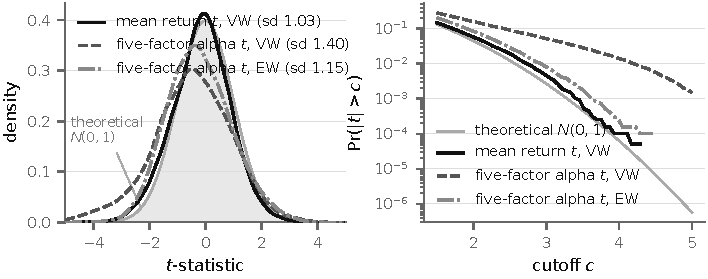
\includegraphics[width=\linewidth]{figures/null_density}
\caption{The measured null against the theoretical one, on a population that is
null by construction. Left: densities, with the standard normal shaded. Right:
the upper tail. The mean-return $t$-statistic is close to nominal; the
five-factor alpha $t$-statistic, which is what published papers report, is not,
and the gap widens with the cutoff. The empirical curves flatten below about
$5 \times 10^{-5}$, which is the resolution floor of 19{,}380 strategies.}
\label{fig:null-density}
\end{figure}

Two findings. First, for the raw mean-return $t$-statistic the theoretical null
is a good approximation, and equal-weighted it is if anything slightly
conservative: standard deviation \bzoonullMeanSdEw{} rather than 1.00. The
construction imposes an approximate zero-sum constraint across strategies within
a letter position --- every group appears equally often on the long and the
short side --- which shrinks the cross-sectional spread. Value-weighted the
figure is \bzoonullMeanSdVw{}, essentially nominal. This confirms
\citeauthor{chen2025htap}'s qualitative statement and puts a number on it.

Second, the statistic published papers report behaves differently. The
five-factor alpha $t$-statistic has cross-sectional standard deviation
\bzoonullFfSdEw{} equal-weighted and \bzoonullFfSdVw{} value-weighted; against
the nominal 5 percent cutoff, \bzoonullFfExceedVwPct{} percent of no-content
strategies are significant, and at $|t| > 3$ the figure is
\bzooamThreeFfFiveVwPct{} percent against a nominal \bzoonominalThreePct{}
percent. Kurtosis stays near 3 throughout, so this is a scale effect and not a
tail-shape effect --- which is what makes the rescaling of
\S\ref{sec:corrections} sufficient, since a scale effect is correctable by one
number and a tail effect is not. Generalised Pareto fits to the upper tail and
their threshold-stability diagnostics are in
\texttt{data/results/empirical\_null.json}.
\S\ref{sec:nullfails} explains where that width comes from, and it is not
sampling noise.

\subsection{Is the population really null in raw returns?}

\emph{Null} in this subsection means null in raw returns, which is the premise
everything after it rests on. Section~\ref{sec:nullfails} shows the same
population is emphatically \emph{not} null in factor-model alphas, and that is
the paper's point; the two statements are compatible and the identity
$\hat\alpha = \bar r - \hat\beta'\bar f$ is why.

A referee's first objection is that ticker letters are not neutral: alphabetical
position is documented to affect turnover and valuation \citep{itzkowitz2016}.
We test \bzooalphabetTests{} subgroups --- the four letter positions, three
alphabetical regions of the long leg, and extreme against interior sorts, in
both weightings --- for a systematic non-zero mean, aggregating each subgroup
into one monthly series first and using a stationary block bootstrap over
months, because strategies within a subgroup share months and are strongly
dependent. Every interval contains zero, and no subgroup is flagged at any
multiplicity correction we apply. Dropping every strategy whose sort touches the extreme ends
of the alphabet leaves the calibration unchanged
(Table~\ref{tab:robustness}). The aggregate mean of the whole ticker population
is \bzootickerMeanEw{} percent per month, $t = \bzootickerMeanTEw$.

Recalibrating separately on the four disjoint letter-position subsets gives a
standard deviation of the mean-return $t$-statistic in the range
\bzoosubpopSdLowEw{} to \bzoosubpopSdHighEw{} equal-weighted, and of the
five-factor alpha $t$-statistic \bzoosubpopFfSdLowVw{} to
\bzoosubpopFfSdHighVw{} value-weighted. The calibration is reproducible in sign
and rough magnitude on 4{,}845 dependent strategies and not to two decimal
places, and we report it as a range.

\subsection{Where the known-null assumption fails}
\label{sec:nullfails}

The wide five-factor null is not a miscalibrated standard error. It is a real
non-zero alpha, and the reason is arithmetic. Ordinary least squares gives
$\hat\alpha = \bar r - \hat\beta' \bar f$ exactly, so a strategy with zero
expected return and non-zero factor loadings has a non-zero alpha. Sorting
stocks on a ticker letter produces no expected return but does produce factor
exposure, because the alphabet is not independent of firm characteristics.

The identity turns into an exact variance decomposition, which is the cleanest
way to say how much dispersion risk adjustment adds:
\begin{equation}
\label{eq:decomp}
\operatorname{Var}(\hat\alpha)
  = \operatorname{Var}(\bar r)
  + \operatorname{Var}(\hat\beta'\bar f)
  - 2\operatorname{Cov}(\bar r,\, \hat\beta'\bar f).
\end{equation}
Value-weighted, in squared basis points per month, the three measured terms are
$\operatorname{Var}(\bar r) = \bzooamVarRbarVw$,
$\operatorname{Var}(\hat\beta'\bar f) = \bzooamVarExposureVw$ and
$\operatorname{Cov}(\bar r, \hat\beta'\bar f) = \bzooamCovTermVw$, which give
$\operatorname{Var}(\hat\alpha) = \bzooamVarAlphaVw$. The covariance is
negative, so the $-2\operatorname{Cov}$ term \emph{adds}
\bzooamVarCovTermVw{} rather than subtracting: strategies with more positive
exposure tend to have lower mean returns, and risk adjustment pulls those two
apart instead of letting them offset. The alphas end up \bzooamSdRatioVw{} times
as dispersed as the mean returns, with \bzooamIncreaseExposurePct{} percent of
the increase coming from the exposure variance and
\bzooamIncreaseCovPct{} percent from the covariance term. Every term is
measured, the identity holds to machine precision, and none of it depends on a
distributional assumption.

A negative covariance in a population that is null by construction invites two
objections, and working through them says something useful about what the term
is. The first is that $\hat\beta$ and $\bar r$ are estimated on the same
months, so the two might be coupled mechanically. They are not: for least
squares with an intercept the coupling term is proportional to the sum of the
demeaned regressor and is therefore exactly zero, with or without
cross-sectional dependence in the residuals. Estimating $\beta$ on the first
half of the sample and forming the exposure on the second, so that the two
sides use disjoint data, leaves the covariance negative at \bzooamCovOosBps{}
squared basis points with a 95 percent bootstrap interval of
\bzooamCovOosLoBps{} to \bzooamCovOosHiBps{}.

The second objection is that a null population should have no such covariance
at all. That is not what the algebra says. Substituting
$\bar r = \beta'(\bar f - \mu_f) + \bar e$ gives
$\operatorname{Cov}_i(\bar r, \beta'\bar f) =
(\bar f - \mu_f)' \Sigma_\beta \bar f$, a realised quadratic form in the sample
factor means whose expectation over samples is
$\operatorname{tr}(\Sigma_\beta \operatorname{Var}(\bar f)) > 0$ and which can
land either side of zero in any one sample. So the sign here is not evidence
that the population fails to be null, and it is not an artefact. It is a
sample-specific realisation --- the same conclusion the variance split of
\S\ref{sec:corrections} reaches from a different direction, and the reason we
do not build any claim on the covariance term's sign.

Two conventions in this literature deserve a correction here, because both are
easy to state and wrong. First, the cross-sectional regression of $\hat\alpha$
on $-\hat\beta'\bar f$ is sometimes said to have a population slope of exactly
one, on the grounds that $\bar r$ is centred at zero. Centring fixes the
\emph{mean} of $\bar r$ and the slope depends on its \emph{covariance}:
substituting the identity gives
$1 + \operatorname{Cov}(\bar r, -\hat\beta'\bar f)/\operatorname{Var}(\hat\beta'\bar f)$.
We measure \bzooamSlopeVw{} value-weighted (White standard error
\bzooamSlopeSeVw{}) and \bzooamSlopeEw{} equal-weighted, and the formula
reproduces both to machine precision. Second, the correlation between
$\hat\alpha$ and $-\hat\beta'\bar f$, \bzooexposureCorrVw{} value-weighted, and
the share $\operatorname{Var}(\hat\beta'\bar f)/\operatorname{Var}(\hat\alpha)$,
\bzooexposureVarShareVwPct{} percent, are different quantities and do not have
to agree: the first squares to \bzooamCorrSquaredVw{} and the gap between them
is exactly the covariance term in~\eqref{eq:decomp}. We report the decomposition rather than
either summary alone.

The standard errors are not doing the work. Across the six specifications of
Table~\ref{tab:across-models} --- the raw mean return and five factor models
--- the median SE$(\hat\alpha)$ moves from
\bzooamMedSeRawVw{} to \bzooamMedSeFfFiveVw{} basis points, about a percent,
while SD$(\hat\alpha)$ moves from \bzooamSdAlphaRawVw{} to
\bzooamSdAlphaFfFiveVw{}. The exact finite-sample cost of estimating $\beta$
rather than knowing it is
$\sqrt{1 + \bar f' S_f^{-1}\bar f} = \bzooamSeInflFfFive{}$ for the five-factor
model --- a squared-Sharpe-ratio quantity that does not shrink with $T$ --- and
it works in the direction that makes $t$ \emph{smaller}, so the widening we
report is a lower bound.

So ``no economic content'' implies a null raw return and does \emph{not} imply a
null alpha.

\subsection{Two questions, two nulls}
\label{sec:twonulls}

Which question a null is for now becomes the whole issue, because the answer
differs and the two are routinely reported as though they were one object.

If the question is \emph{does this strategy have a non-zero alpha} --- a test of
$\alpha = 0$ --- then the marginal cross-sectional spread of the ticker
population is the wrong null, for exactly the reason just given: these alphas
are genuinely non-zero, so their spread is not the distribution of $\hat\alpha$
under $\alpha = 0$ but the distribution of a real quantity. The right null is
one that imposes $\alpha = 0$ while leaving the exposures where they are. We
construct it by sign-flipping the factor-model residuals in blocks, with the
same sign vector across all strategies, which leaves the loadings and the
cross-strategy dependence untouched. That gives a 95th percentile of the largest
alpha $t$-statistic of \bzooffMaxTJointVw{} value-weighted, against
\bzooffMaxTIndepVw{} with dependence removed, and those are the numbers
\S\ref{sec:thresholds} uses.

If the question is \emph{does this signal have content} --- which is what a
researcher screening candidate signals is actually asking --- then the marginal
spread is precisely the right object, and the fact that the alphas are real is
what makes it so. It answers: what alpha $t$-statistics do empty-but-exposed
strategies produce? A screener needs to clear that distribution, not a
distribution built by assuming away the exposure that the empty strategies
actually have. Its 95th percentile, \bzooamCutoffFfFiveVw{} value-weighted, is
the cutoff we recommend in \S\ref{sec:remedy}, and it is a screening
calibration rather than a hypothesis test.

The two nulls answer different questions and neither substitutes for the other.
A signal can have a genuinely non-zero alpha --- passing the first test --- and
still be indistinguishable from a ticker sort --- failing the second. That
combination is not a contradiction; it is the entire phenomenon this paper
describes.

\subsection{Four checks on the mechanism, and where the exposure comes from}
\label{sec:mechanism}

% generated by bzoo.report.tables on 2026-08-01; do not edit by hand
\begin{table}[t]
\centering
\caption{Dose-response across benchmark models, on the 19{,}380 ticker strategies. $K$ is the number of factors; every row is the same strategies over the same 714 months, so only the model changes. SD($\hat\alpha$) and the median standard error are in basis points per month. \emph{SE infl.} is $\sqrt{1+\bar f'S_f^{-1}\bar f}$, the exact finite-sample cost of estimating $\beta$ rather than knowing it, which is a Sharpe-ratio quantity and does not shrink with $T$. The spread of the alpha widens by a third while the standard error moves by about a percent, so the widening is entirely in the numerator.}
\label{tab:across-models}
\begin{tabular}{lrrrrrrrrrrr}
\toprule
\textbf{Model} & \textbf{$K$} & \textbf{Wt.} & \textbf{SD} & \textbf{MAD-SD} & \textbf{Kurt.} & \textbf{$\Pr(|t|>1.96)$} & \textbf{$\Pr(|t|>3)$} & \textbf{5\% cutoff} & \textbf{SD($\hat\alpha$)} & \textbf{Med. SE} & \textbf{SE infl.} \\
\midrule
Raw mean return & 0 & VW & 1.023 & 0.985 & 3.09 & 0.0618 & 0.0044 & 2.07 & 9.43 & 7.96 & 1.0000 \\
CAPM & 1 & VW & 1.070 & 1.066 & 2.96 & 0.0724 & 0.0053 & 2.14 & 9.97 & 7.95 & 1.0076 \\
Fama--French 3 & 3 & VW & 1.361 & 1.362 & 2.93 & 0.1658 & 0.0345 & 2.79 & 12.31 & 7.88 & 1.0173 \\
Carhart 4 & 4 & VW & 1.283 & 1.287 & 2.96 & 0.1377 & 0.0248 & 2.62 & 12.06 & 8.03 & 1.0398 \\
Fama--French 5 & 5 & VW & 1.405 & 1.342 & 3.30 & 0.1674 & 0.0523 & 3.04 & 13.11 & 8.00 & 1.0465 \\
FF5 + momentum & 6 & VW & 1.368 & 1.283 & 3.42 & 0.1549 & 0.0467 & 2.92 & 12.97 & 8.10 & 1.0628 \\
\midrule
Raw mean return & 0 & EW & 0.883 & 0.888 & 2.82 & 0.0292 & $5.160\times 10^{-5}$ & 1.76 & 4.58 & 4.70 & 1.0000 \\
CAPM & 1 & EW & 0.883 & 0.905 & 2.73 & 0.0446 & 0.0001 & 1.92 & 4.94 & 4.71 & 1.0076 \\
Fama--French 3 & 3 & EW & 0.909 & 0.940 & 2.74 & 0.0331 & $5.160\times 10^{-5}$ & 1.82 & 4.73 & 4.68 & 1.0173 \\
Carhart 4 & 4 & EW & 0.941 & 0.974 & 2.72 & 0.0332 & 0.0002 & 1.83 & 5.02 & 4.78 & 1.0398 \\
Fama--French 5 & 5 & EW & 1.150 & 1.151 & 2.97 & 0.0915 & 0.0082 & 2.27 & 5.99 & 4.76 & 1.0465 \\
FF5 + momentum & 6 & EW & 1.213 & 1.223 & 2.93 & 0.1232 & 0.0143 & 2.45 & 6.54 & 4.83 & 1.0628 \\
\bottomrule
\end{tabular}
\end{table}


\paragraph{Across benchmark models.}
Table~\ref{tab:across-models} and the left panel of
Figure~\ref{fig:across-models} run the same strategies over the same months
under the raw mean return and five factor models. Value-weighted,
SD$(t_\alpha)$ goes
\bzooamSdRawVw{}, \bzooamSdCapmVw{}, \bzooamSdFfThreeVw{},
\bzooamSdCarhartVw{}, \bzooamSdFfFiveVw{}, \bzooamSdFfSixVw{} for
$K = 0,1,3,4,5,6$. It is not monotone in $K$, and it should not be: what
matters is not how many regressors are added but whether the added factor
carries a mean return the sort happens to load on. Adding momentum to
Fama--French 3 lowers the spread; adding profitability and investment raises
it. A count of regressors does not predict the curve and the exposures do.

% generated by bzoo.report.tables on 2026-09-21; do not edit by hand
\begin{table}[t]
\centering
\caption{Within-population dose-response, value-weighted. Strategies are sorted into deciles by the absolute size of their exposure term $|\hat\beta'\bar f|$; all quantities except the last two are in basis points per month. Across the deciles the numerator of the $t$-statistic rises by a factor of two while its denominator rises by a fifth, which is what identifies the mechanism as exposure rather than a standard-error effect. The bottom decile is a within-population placebo: strategies with almost no exposure have an alpha $t$-statistic of almost exactly the textbook width.}
\label{tab:exposure-deciles}
\begin{adjustbox}{max width=\linewidth}
\begin{tabular}{lrrrrrrr}
\toprule
\textbf{Decile} & \textbf{$n$} & \textbf{Median $|\hat\beta'\bar f|$} & \textbf{SD($t_\alpha$)} & \textbf{SD($\hat\alpha$)} & \textbf{Median SE($\hat\alpha$)} & \textbf{$\Pr(|t_\alpha|>3)$} & \textbf{Median $R^2$} \\
\midrule
1 & 1938 & 0.48 & 0.994 & 8.88 & 7.64 & 0.0031 & 0.049 \\
2 & 1938 & 1.43 & 1.013 & 9.06 & 7.67 & 0.0052 & 0.047 \\
3 & 1938 & 2.41 & 1.025 & 9.21 & 7.67 & 0.0046 & 0.047 \\
4 & 1938 & 3.42 & 1.084 & 9.71 & 7.73 & 0.0103 & 0.049 \\
5 & 1938 & 4.53 & 1.126 & 10.21 & 7.79 & 0.0160 & 0.051 \\
6 & 1938 & 5.73 & 1.250 & 11.36 & 7.88 & 0.0237 & 0.055 \\
7 & 1938 & 7.14 & 1.309 & 12.16 & 8.04 & 0.0310 & 0.059 \\
8 & 1938 & 8.91 & 1.486 & 13.62 & 8.18 & 0.0630 & 0.068 \\
9 & 1938 & 11.22 & 1.646 & 15.19 & 8.45 & 0.1202 & 0.078 \\
10 & 1938 & 15.66 & 1.810 & 17.59 & 9.11 & 0.2461 & 0.099 \\
\bottomrule
\end{tabular}
\end{adjustbox}
\end{table}


\begin{figure}[t]
\centering
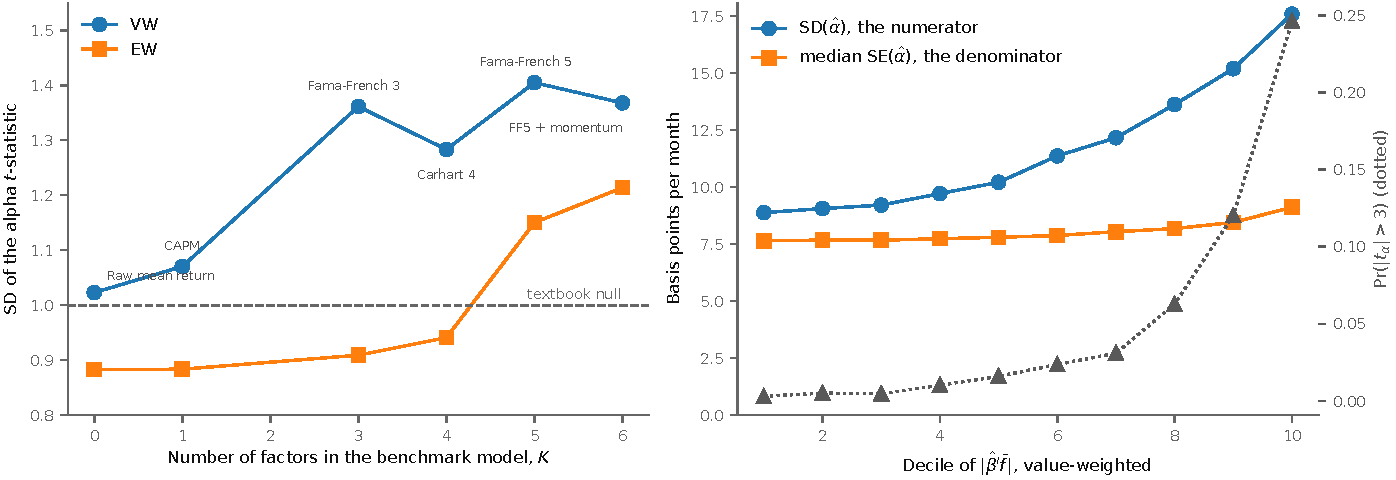
\includegraphics[width=\linewidth]{figures/across_models}
\caption{Left: the spread of the alpha $t$-statistic on a population with no
predictive content, under the raw mean return and five factor models. Right:
within the
value-weighted population, sorted into deciles by exposure. The numerator of
the $t$-statistic rises across the deciles by a factor of
\bzooamDecileNumeratorRatio{} and the denominator by
\bzooamDecileDenominatorRatio{}, which is what makes this an exposure effect
rather than a standard-error effect.}
\label{fig:across-models}
\end{figure}

\paragraph{Within the population.}
Table~\ref{tab:exposure-deciles} sorts the strategies into deciles on
$|\hat\beta'\bar f|$. SD$(t_\alpha)$ runs from \bzooamDecileOneSd{} in the
bottom decile to \bzooamDecileTenSd{} in the top, and $\Pr(|t_\alpha|>3)$ from
\bzooamDecileOneThreePct{} percent to \bzooamDecileTenThreePct{} percent. The
bottom decile is a placebo drawn from inside the population itself: strategies
that happen to carry almost no exposure have an alpha $t$-statistic of almost
exactly the textbook width. Binning on $R^2$ instead gives a similar picture
for a reason that is partly a denominator effect --- a higher $R^2$ means a
smaller residual variance and a smaller standard error --- which is why the
exposure binning is the one we lead with, and why SD$(\hat\alpha)$ is reported
next to SD$(t_\alpha)$ in every bin.

\paragraph{A zero-exposure placebo.}
Simulating returns with zero mean and zero population exposure, matched to each
strategy's residual volatility, and running the identical five-factor
regressions gives SD$(t_\alpha) = \bzooamPlaceboIid$ under independent normal
draws and \bzooamPlaceboBoot{} under a bootstrap of the fitted residuals that
preserves their dependence and non-normality. The regression machinery does
not manufacture the spread; the exposures do.

\begin{figure}[t]
\centering
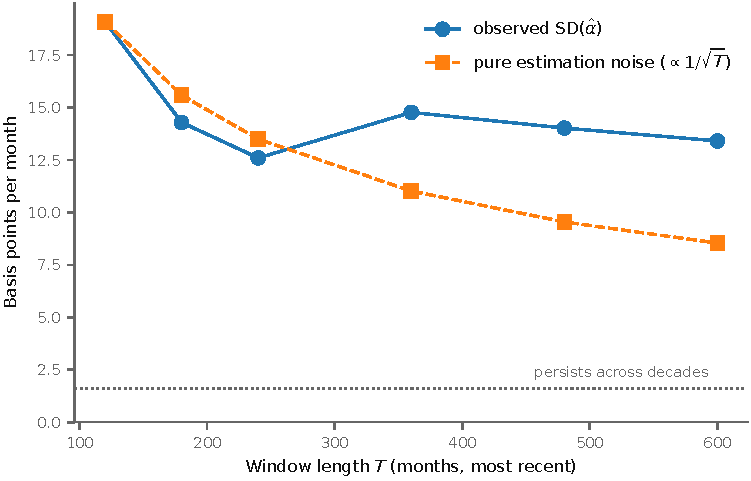
\includegraphics[width=0.55\linewidth]{figures/exposure_dose_response}
\caption{The dispersion of $\hat\alpha$ over nested windows of the most recent
$T$ months, against what pure estimation noise would give. The dotted line is
the component that persists across disjoint decades, estimated separately, and
it is far below the gap between the two curves: most of that gap is
period-specific exposure rather than a fixed property of the strategy.}
\label{fig:persistence}
\end{figure}

\paragraph{Persistence, and what does \emph{not} persist.}
A spread that is pure estimation noise shrinks like $1/\sqrt{T}$. This one does
not: over nested windows the observed dispersion of $\hat\alpha$ falls from
\bzooamObservedAlphaBpsShort{} to \bzooamObservedAlphaBpsLong{} basis points
where noise alone would
predict \bzooamNoiseOnlyAlphaBps{}, which is the right panel of
Figure~\ref{fig:persistence}. That curve is descriptive only, and we do not
fit it: nested windows share most of their data, so the points are heavily
dependent and any standard error on a fitted intercept would be
uninterpretable.

The question the curve raises --- is there a component of these alphas that is
a fixed property of the strategy rather than of the sample --- has a clean
answer that needs no functional form. Split the sample into \bzooamNBlocks{}
disjoint \bzooamBlockMonths{}-month blocks and estimate every strategy's alpha
separately in each. Estimation noise is independent across disjoint blocks, so
it inflates the within-block cross-sectional variance and contributes nothing
to the covariance between two different blocks; the between-block covariance is
therefore an unbiased estimate of the persistent variance on its own. Bootstrapping
over strategies, that component is \bzooamPersistentBps{} basis points per
month, 95 percent interval \bzooamPersistentLoBps{} to
\bzooamPersistentHiBps{}, against a within-block dispersion of
\bzooamWithinBlockSdBps{} basis points.

So it is different from zero --- \bzooamPersistentBootP{} of the bootstrap
distribution lies below zero, a one-sided level of the same size --- and it is
small, only
\bzooamPersistentSharePct{} percent of the within-block variance. We read that
as follows, and it is the more interesting reading. The inflated alphas are
real in any given sample, which is what defeats a multiplicity correction. They
are largely \emph{not} stable across decades, because the exposure term
$\hat\beta'\bar f$ depends on realised factor premia and those move. A screener
who finds one of these has therefore found neither a chance result nor a
durable anomaly, but a sample-specific exposure artefact --- and both halves of
that are bad news, because the first means a stricter threshold will not remove
it and the second means it will not replicate.

\paragraph{Where the exposure comes from, and what wins.}
Decomposing $\hat\beta'\bar f$ by factor, the investment and profitability
terms carry \bzooamShareRmwCmaPct{} percent of its variance, size
\bzooamShareSmbPct{} percent and the market only \bzooamShareMktPct{} percent.
The story is not the size effect one might guess from
\citet{itzkowitz2016}: size carries \bzooamShareSmbPct{} percent and the two
factors that dominate are the ones Fama and French added in 2015.

We cannot say why. Letter position and the alphabet regions of the two legs
explain $R^2 = \bzooamAlphabetRsq$ of the exposure, so the alphabet does map
systematically onto profitability and investment loadings, but weakly, and a
weak reduced-form mapping is not a mechanism. The candidate we would test first
is industry: firms have historically chosen mnemonic tickers, so ticker letters
should cluster by sector, and sector composition would plausibly drive
profitability and investment loadings. Testing it needs the industry
composition of each long leg, which needs firm-level holdings; \citet{chen2025htap}
distribute portfolio returns only, so it needs CRSP identifiers and SIC codes
that are outside what this paper's data allows. We flag it as the obvious next
step rather than gesturing at it as though it were established. In the top and bottom one
percent of alphas the loadings flip sign as the mechanism requires: the
strategies with the largest positive alphas are the ones short the priced
factors. The single most significant strategy value-weighted is \bzooamWinnerName{} ---
sort on the second letter of the ticker, buy two groups and sell two others.
Its three numbers are $\bar r = \bzooamWinnerRbarBps$,
$\hat\beta'\bar f = \bzooamWinnerExposureBps$ and therefore
$\hat\alpha = \bzooamWinnerAlphaBps$ basis points per month. Losing
\bzooamWinnerRbarBps{} while carrying enough exposure to have been expected to
make \bzooamWinnerExposureBps{} gives $t_\alpha = \bzooamWinnerAlphaT$, which
clears Bonferroni at the full trial count, on a raw-return $t$-statistic of
\bzooamWinnerMeanT{}. \bzooamWinnerExposureSharePct{} percent of the alpha is
the exposure, and the strategy has no content at all.

\subsection{A second no-content population}

% generated by bzoo.report.tables on 2026-08-01; do not edit by hand
\begin{table}[t]
\centering
\caption{Two no-content populations, built differently, widened the same way. Dispersions of $\bar r$ and $\hat\alpha$ are in basis points per month; each \emph{Ratio} column is the alpha entry divided by the mean-return entry to its left. The second population's alpha $t$-statistics sit near the textbook width in \emph{absolute} terms only because its raw-return null is unusually narrow to begin with: risk adjustment widens its numerator by as much as it widens the ticker population's. Two independent constructions, one mechanism.}
\label{tab:alt-population}
\begin{tabular}{lrrrrrrrr}
\toprule
\textbf{Population} & \textbf{Wt.} & \textbf{$n$} & \textbf{SD($t_{\bar r}$)} & \textbf{SD($t_\alpha$)} & \textbf{Ratio} & \textbf{SD($\bar r$)} & \textbf{SD($\hat\alpha$)} & \textbf{Ratio } \\
\midrule
Ticker letters & VW & 19\,380 & 1.023 & 1.405 & 1.373 & 9.43 & 13.11 & 1.390 \\
Higher-moment, 3--5 yr & VW & 210 & 0.775 & 1.009 & 1.301 & 8.08 & 11.48 & 1.420 \\
Ticker letters & EW & 19\,380 & 0.883 & 1.150 & 1.303 & 4.58 & 5.99 & 1.308 \\
Higher-moment, 3--5 yr & EW & 210 & 0.663 & 0.887 & 1.338 & 5.50 & 6.57 & 1.194 \\
\midrule
\bottomrule
\end{tabular}
\end{table}


The \bzooamAltN{} higher-moment past-return strategies built only from returns
three to five years old --- a different construction, with no documented effect
at that horizon --- give an independent test.  Value-weighted their five-factor
alpha $t$-statistic has standard deviation \bzooamAltSdAlphaTVw{}, against the
ticker population's \bzoonullFfSdVw{}, and it would be easy to read that as the
alpha inflation being specific to ticker sorts. It is not, and
Table~\ref{tab:alt-population} shows why. That population's \emph{raw-return}
null is unusually narrow, \bzooamAltSdMeanTVw{}, so the right comparison is not
the level but the widening. Risk adjustment multiplies the dispersion of this
population's numerator by \bzooamAltWideningVw{} and the ticker population's by
\bzooamTickerWideningVw{}. Two populations built from unrelated sorting
variables, widened by the same amount. The mechanism replicates.

The transferable lesson is the general form: a population that is null with
respect to one statistic need not be null with respect to a transformation of
it, and any signal that induces factor exposure without predictive content will
produce inflated alpha $t$-statistics. That is a real false-discovery channel
for anyone screening signals on risk-adjusted statistics, and because the
alphas are real rather than spurious, no multiplicity correction addresses it.

\paragraph{What would overturn this.} Four results would, and we report all
four rather than only the ones that came out our way. \emph{One}: a no-content
population that carries factor exposure but shows no alpha inflation. Our
second population is such a test and it inflates
(Table~\ref{tab:alt-population}). \emph{Two}: a zero-exposure simulation
returning SD$(t_\alpha)$ materially above 1. It returns \bzooamPlaceboIid{}.
\emph{Three}: no relationship between exposure and alpha inflation within a
population. The relationship is monotone across all ten deciles and the
numerator carries it (Table~\ref{tab:exposure-deciles}). \emph{Four}: alpha
dispersion shrinking exactly like $1/\sqrt{T}$, which would make it estimation
noise; it does not, and a disjoint-block estimate puts a small but non-zero
persistent component at \bzooamPersistentBps{} basis points. Two of the checks we ran did not
behave as the simple version of the theory predicts --- SD$(t_\alpha)$ is not
monotone in the number of factors, and the cross-sectional slope of
$\hat\alpha$ on $-\hat\beta'\bar f$ is \bzooamSlopeVw{} rather than 1 --- and
in both cases the identity predicts the departure exactly, which is reported
above.

\subsection{What a correction does and does not fix}
\label{sec:corrections}

% generated by bzoo.report.tables on 2026-08-01; do not edit by hand
\begin{table}[t]
\centering
\caption{Multiplicity corrections applied to 19{,}380 strategies that have no economic content by construction, value-weighted, with the family size set to the full 19{,}380 and the nominal standard normal used as the null. Every rejection in this table is a false one. A 5 percent family-wise procedure promises at most a 5 percent chance of \emph{any} rejection across the family; on the raw mean return Bonferroni delivers that and rejects nothing, and on the five-factor alpha it rejects 69 times. The multiplicity arithmetic is not what fails --- the null it is applied to is.}
\label{tab:corrections-on-null}
\begin{tabular}{lrr}
\toprule
\textbf{Correction} & \textbf{Mean return $t$} & \textbf{Five-factor $\alpha$ $t$} \\
\midrule
Uncorrected ($|t|>1.96$) & 1\,197 & 3\,244 \\
Bonferroni & 0 & 69 \\
\v{S}id\'ak & 0 & 70 \\
Holm & 0 & 69 \\
Benjamini--Hochberg & 0 & 995 \\
Benjamini--Yekutieli & 0 & 292 \\
\bottomrule
\end{tabular}
\end{table}


The claim that a multiplicity correction is no remedy here is directly
testable, and Table~\ref{tab:corrections-on-null} is the test: apply the
corrections to a population where every rejection is by construction a false
one. A 5 percent family-wise procedure promises at most a 5 percent chance of
\emph{any} rejection across the family. On the raw mean-return $t$-statistic
Bonferroni delivers exactly that and rejects \bzooamBonfFalseMean{} of
19{,}380. On the five-factor alpha, at the same family size and the same
nominal null, it rejects \bzooamBonfFalseAlpha{}. Benjamini--Hochberg rejects
\bzooamBhFalseAlpha{} against \bzooamBhFalseMean{}. Same strategies, same
correction, same $M$; the only thing that changed is the statistic.

It is not the multiplicity arithmetic that fails. Substituting the measured
null for the standard normal --- keeping Bonferroni and keeping
$M = 19{,}380$, and only widening the null from 1.00 to \bzoonullFfSdVw{} ---
moves the critical value from \bzooamBonfCrit{} to \bzooamMeasuredBonfCrit{}
and the false rejections from \bzooamBonfFalseAlpha{} to
\bzooamMeasuredBonfFalse{}. The correction works once it is given the right
null. What it cannot do is supply that null itself.

\paragraph{Why a fixed rescaling is enough, and where it stops.}
This deserves an explanation rather than a lucky observation, and the identity
supplies one. For a strategy with no content the true alpha is
$-\beta'\mu_f$, using population premia, while the estimate is
$\hat\alpha = -\beta'\mu_f - \beta'(\bar f - \mu_f) + \bar e + O(1/T)$. The two
middle terms behave completely differently in $t$-units. The first is a fixed
quantity divided by a standard error that shrinks like $1/\sqrt{T}$, so it
contributes a variance growing like $T$. The second involves $\bar f - \mu_f$,
which converges at exactly the rate the standard error shrinks, so it
contributes a variance that does not grow at all. Writing
$\operatorname{Var}(t_\alpha) = 1 + c_1 + c_2 T$, the persistent piece is
$c_2 T$ and the sample-specific piece is $c_1$.

We can separate them, because the disjoint-block estimate of
\S\ref{sec:mechanism} measures $\operatorname{Var}(\beta'\mu_f)$ directly.
Value-weighted, $c_1 = \bzooamCOne$ and $c_2 T = \bzooamCTwoT$ at
$T = 714$: \bzooamCOneSharePct{} percent of the excess variance is the
sample-specific term and \bzooamCTwoSharePct{} percent is the growing one. The
sample length at which the growing term would matter as much as the fixed one
is about \bzooamTEqualYears{} years. That is why rescaling works, and it is the
honest reason: on any sample a researcher will ever have, this channel is a
fixed variance inflation rather than a divergence.

\paragraph{What survives.} Three things, and they are what the paper claims.
A correction applied with the \emph{nominal} null does not address this channel
at any family size --- with fifty candidate signals, Bonferroni still gives
\bzooamFamFiftyBonf{} expected false positives and a
\bzooamFamFiftyAnyPct{} percent chance of at least one, against the 5 percent
it promises, and even with ten candidates the chance is
\bzooamFamTenAnyPct{} percent. A correction applied with a \emph{measured}
null does address it, but the measurement is the hard part: the inflation is a
property of the candidate population's exposure distribution, so it has to be
estimated on the population being screened rather than borrowed from this one.
And a residual component does grow with the sample, so no fixed threshold
contains it forever, though on realistic samples that component is small.

\subsection{Dependence, and why the effective test count is the wrong summary}
\label{sec:dependence}

Dependence is measured with the marginals held exactly fixed. A block sign-flip
permutation applied to the whole cross-section at once gives the null
distribution of $\max_k |t_k|$ with dependence intact; the same permutation with
an independent sign vector per strategy gives the same marginals with the
columns independent. On \bzoonStrategiesComplete{} complete-history strategies
the 95th percentile of $\max_k |t_k|$ is \bzoomaxTJoint{} jointly and
\bzoomaxTIndep{} independently: dependence lowers the threshold by
\bzoodependenceMovePct{} percent.

Converting that into an effective number of independent tests is where the
literature's usual summary breaks down. On the same correlation matrix,
\citet{cheverud2001} and \citet{nyholt2004} give \bzoonEffCheverud{} and
\citet{liji2005} gives \bzoonEffLiJi{}, out of
\bzoonStrategiesComplete{} --- a disagreement of two orders of magnitude. The
\citeauthor{sidak1967}-implied count from the permutation maximum sits between
them. The instability is not a defect of any one estimator: $N_{\text{eff}}$ is
an exponentially amplified rescaling of a threshold, so the
\bzoodependenceMovePct{} percent move measured above is a three- to five-fold
move in the count. We therefore report the maximum-statistic quantile as the
primary object and the effective count as a derived quantity, and we recommend
that others do the same.

% ==========================================================================
\section{Thresholds, and the published predictors}
\label{sec:thresholds}

Table~\ref{tab:thresholds} puts five thresholds for the same family of tests on
one scale, and Figure~\ref{fig:thresholds} shows them.

% generated by bzoo.report.tables on 2026-09-21; do not edit by hand
\begin{table}[t]
\centering
\caption{Five thresholds for the same family of tests, on one scale. \emph{Nominal} is 1.96. \emph{Calibrated} is the 95th percentile of the measured null for a single test. \emph{Bonferroni} applies the nominal null with $M = 14{,}535$, the number of strategies with a complete 720-month history; the fourth ticker letter position exists only for the most recent 600 months, which is why that count is three quarters of the 19{,}380 and not all of them. The two max-$t$ columns are the 95th percentile of the null maximum with the measured marginals, without and with cross-strategy dependence; the second is correct. \emph{Bonf.\ error} is how much Bonferroni overshoots it. The two alpha rows mix two constructions and should be read as such: \emph{Null SD} and \emph{Calibrated} come from the marginal cross-sectional spread, which Section~\ref{sec:nullfails} shows is not a null, while the max-$t$ columns come from the permutation that imposes $\alpha = 0$ given the exposures. Only the latter is used as a threshold.}
\label{tab:thresholds}
\begin{adjustbox}{max width=\linewidth}
\begin{tabular}{llrrrrrrr}
\toprule
\textbf{Statistic} & \textbf{Wt.} & \textbf{Null SD} & \textbf{Nominal} & \textbf{Calibrated} & \textbf{Bonferroni} & \textbf{Max-$t$ indep.} & \textbf{Max-$t$ joint} & \textbf{Bonf. error} \\
\midrule
Mean return $t$ & EW & 0.889 & 1.96 & 1.77 & 4.64 & 4.73 & 4.39 & 0.057 \\
Five-factor alpha $t$ & EW & 1.150 & 1.96 & 2.27 & 4.64 & 4.35 & 4.12 & 0.127 \\
Mean return $t$ & VW & 1.026 & 1.96 & 2.08 & 4.64 & 4.57 & 4.31 & 0.078 \\
Five-factor alpha $t$ & VW & 1.405 & 1.96 & 3.04 & 4.64 & 4.33 & 4.09 & 0.134 \\
\bottomrule
\end{tabular}
\end{adjustbox}
\end{table}


\begin{figure}[t]
\centering
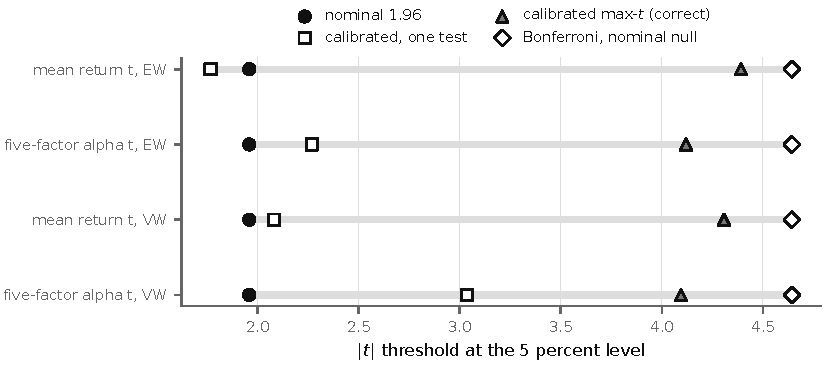
\includegraphics[width=\linewidth]{figures/thresholds}
\caption{Five thresholds for one family of tests. Bonferroni with the raw trial
count lands \bzoobonfErrorMeanEwPct{} percent above the correct calibrated
maximum for the equal-weighted mean-return statistic and
\bzoobonfErrorFfVwPct{} percent above it for the value-weighted five-factor
alpha. The uncorrected 1.96 is more than a factor of two below the correct
threshold in every row.}
\label{fig:thresholds}
\end{figure}

Bonferroni with the raw trial count comes within
\bzoobonfErrorMeanEwPct{} percent of the correct calibrated maximum for the
mean-return $t$-statistic, and it overshoots by \bzoobonfErrorFfVwPct{} percent
for the five-factor alpha. It overshoots on both, and for two reasons that
compound rather than cancel: it ignores dependence, which would lower the
correct threshold, and it assumes a standard normal marginal that is
\emph{wider} and heavier-tailed than the measured one for the mean-return
statistic --- SD \bzoonullMeanSdEw{} and kurtosis \bzoonullMeanKurtEw{}
equal-weighted --- which would lower it again. The margin is small on the mean
return only because both effects are small there. The practical reading is that the conventional
correction is close to right for the raw mean return and noticeably too strict
for the factor-model alpha, and that in neither case does it get there by the
route its user would describe.

\paragraph{The published predictors, briefly.}
Re-evaluating the \bzoopublishedN{} published predictors on their own original
windows, \bzoopublishedShareTwoPct{} percent clear 1.96 uncorrected, Bonferroni
leaves \bzoosurvBonfNominal{} and Benjamini--Hochberg \bzoosurvBhNominal{};
calibrating the null on the ticker population makes \emph{more} of them
survive, \bzoosurvBonfCalibrated{} and \bzoosurvBhCalibrated{}. We report this
in one paragraph rather than as a finding, for two reasons that both point the
same way. The measured null is narrow largely because of the zero-sum
constraint of \S\ref{sec:null} --- within a letter position every group appears
equally often long and short --- and a published predictor is under no such
constraint, so transporting this null to that population is exactly the mistake
\S\ref{sec:remedy} warns against. And \citet{chen2025htap} already conclude
that this literature's multiple-testing methods are too strict, so the
direction is a numerical confirmation of theirs rather than a new result. The
full table, the dependence-aware procedures and the
\citet{harvey2015backtesting} haircuts are in
Appendix~\ref{app:survival}.

One caveat applies to every calibrated threshold in this paper. With 19{,}380
strategies the empirical tail resolves no finer than about $5\times 10^{-5}$,
so a calibrated cutoff past roughly $M = 200$ is a Gaussian extrapolation from
the measured null rather than a measured quantile. We report it because the
extrapolation is the same one Bonferroni makes and the comparison is the point,
but it should not be quoted as a measurement.

% ==========================================================================
\section{Robustness}
\label{sec:robust}

% generated by bzoo.report.tables on 2026-09-21; do not edit by hand
\begin{table}[t]
\centering
\caption{Robustness suite. Every entry is reported whatever it shows. For the joint-versus-independent rows a value below one means the correct scheme gives a smaller null maximum, which is the whole point; for the expanding-window rows one is perfect and the nominal null's own errors are in Section~\ref{sec:robust}; for the exclusion and second-population rows the comparison is with the full-population value in Table~\ref{tab:null-summary}. The individual numbers behind every row are in \texttt{data/results/robustness.json}.}
\label{tab:robustness}
\begin{adjustbox}{max width=\linewidth}
\begin{tabular}{p{0.42\linewidth}p{0.30\linewidth}r}
\toprule
\textbf{Check} & \textbf{Quantity} & \textbf{Value} \\
\midrule
Joint vs independent resampling, finance & max-$|t|$ 95th pct ratio & 0.920 \\
Joint vs independent resampling, cora & $\sigma_\Delta$ ratio & 0.874 \\
Joint vs independent resampling, citeseer & $\sigma_\Delta$ ratio & 0.796 \\
Joint vs independent resampling, pubmed & $\sigma_\Delta$ ratio & 0.799 \\
Joint vs independent resampling, ogbn-arxiv & $\sigma_\Delta$ ratio & 0.820 \\
Block length 1 to 12 & spread in max-$|t|$ 95th pct (\%) & 4.322 \\
Expanding window, EW, cutoff 1.96 & observed / predicted, calibrated & 0.625 \\
Expanding window, EW, cutoff 2.5 & observed / predicted, calibrated & 0.624 \\
Expanding window, EW, cutoff 3.0 & observed / predicted, calibrated & 0.361 \\
Expanding window, VW, cutoff 1.96 & observed / predicted, calibrated & 1.898 \\
Expanding window, VW, cutoff 2.5 & observed / predicted, calibrated & 2.160 \\
Expanding window, VW, cutoff 3.0 & observed / predicted, calibrated & 1.058 \\
Second null population, EW & SD of mean-return $t$ & 0.662 \\
Second null population, VW & SD of mean-return $t$ & 0.779 \\
Drop alphabet-extreme sorts, EW & SD of mean-return $t$ & 0.912 \\
Drop alphabet-extreme sorts, VW & SD of mean-return $t$ & 1.037 \\
Balanced accuracy, cora & $\sigma_\Delta$ ratio to accuracy & 0.994 \\
Balanced accuracy, citeseer & $\sigma_\Delta$ ratio to accuracy & 0.912 \\
Balanced accuracy, pubmed & $\sigma_\Delta$ ratio to accuracy & 0.896 \\
Balanced accuracy, ogbn-arxiv & $\sigma_\Delta$ ratio to accuracy & 0.698 \\
\bottomrule
\end{tabular}
\end{adjustbox}
\end{table}


Six checks, with the underlying numbers in
\texttt{data/results/robustness.json}.

\textbf{Expanding-window calibration, and the one that partly fails.} Read this
one first, because it bounds what the threshold results below are worth. We fit the
null on months before 1995 and ask how well it predicts exceedance rates after
1995. The scale is not stable across the two halves: it falls from
\bzooexpWindowSdEarlyEw{} to \bzooexpWindowSdLateEw{} equal-weighted and rises
from \bzooexpWindowSdEarlyVw{} to \bzooexpWindowSdLateVw{} value-weighted.
Measured as mean absolute log error in the predicted exceedance rate across
cutoffs 1.96, 2.5 and 3.0, the calibrated null scores
\bzooexpWindowErrCalEw{} against the nominal null's \bzooexpWindowErrNomEw{}
equal-weighted, and \bzooexpWindowErrCalVw{} against \bzooexpWindowErrNomVw{}
value-weighted. So calibrating helps out of sample in one weighting and hurts in
the other, and value-weighted it hurts substantially: the calibration
under-predicts the observed exceedance rate by up to a factor of
\bzooexpWindowWorstRatioVw{} across the three cutoffs. We take this as a real limit on how far a single unconditional
calibration can be pushed, consistent with the decade-by-decade spread in
\S\ref{sec:null}. What it bounds is the \emph{threshold} result of
\S\ref{sec:thresholds}, which is the part that requires the calibration to
transfer. It does not bound the mechanism of \S\ref{sec:nullfails}, which is an
algebraic identity plus a measured exposure and needs no calibration to hold in
any period.

\textbf{The other five.} \emph{Alternative population}: the \bzooamAltN{}
higher-moment past-return strategies at horizons with no documented effect give
a second, weaker null, narrower than the ticker population in level on both
statistics but widened by risk adjustment in the same proportion
(\S\ref{sec:mechanism}), which is the check that identified the alpha result as
a general exposure mechanism rather than a quirk of ticker sorts.
\emph{Block length and replicate count}: the calibrated maximum moves by
\bzoobootBlockSpreadPct{} percent across block lengths from 1 to 12, and is
stable to within a percent from 8{,}000 replicates upward.
\emph{Joint against independent resampling}: quantified, and it is the
difference reported in \S\ref{sec:dependence}.
\emph{Alphabet-extreme exclusion}: leaves the calibration unchanged.
\emph{Subperiods and volatility regimes}: reported per decade and per regime.


% ==========================================================================
\section{What to do instead}
\label{sec:remedy}

Three recommendations follow from \S\ref{sec:nullfails}, in increasing order of
how much work they cost.

\textbf{Screen on the statistic that answers the question.} If the question is
whether a signal earns money, the raw mean return answers it and the alpha does
not. On the known-null population $\Pr(|t_{\bar r}| > 3)$ is
\bzooamThreeRawVwPct{} percent against the nominal \bzoonominalThreePct{}
percent, while $\Pr(|t_\alpha| > 3)$ is \bzooamThreeFfFiveVwPct{} percent. The
alpha remains the right statistic for asking whether a strategy beats a
benchmark, which is a different question and one where the exposure term is the
answer rather than a contaminant.

\textbf{Calibrate the cutoff on your own candidate population.} On our
population a value-weighted five-factor alpha needs \bzooamCutoffFfFiveVw{}
rather than 1.96 for a 5 percent per-test false positive rate, and the raw mean
return needs \bzooamCutoffRawVw{}; Table~\ref{tab:across-models} has both for
every model we run. We are deliberately not recommending
\bzooamCutoffFfFiveVw{} as a number to adopt, because this paper contains the
evidence that it does not transfer: the second no-content population has a
different alpha dispersion, and the cutoff follows the exposure distribution
rather than the statistic. The recommendation is the procedure --- form the
population of signals you are willing to have searched, measure the spread of
the statistic you intend to screen on over it, and take the quantile you want.

Two things make our number a floor rather than an estimate. A ticker letter
induces factor exposure \emph{accidentally}, whereas a candidate signal built
from firm characteristics is related to size, value and profitability by
construction, so a realistic search space should carry more exposure than this
one and need a higher cutoff. And the tail resolves no finer than
$5 \times 10^{-5}$ on 19{,}380 strategies, so any cutoff quoted for a family
much past $M = 200$ is an extrapolation.

\textbf{Report both statistics.} A signal whose evidence lives entirely in the
exposure channel clears the alpha bar and not the raw-return bar, and the two
counts together identify it where neither alone does. Recomputing the
\bzooamPubN{} published predictors on their own original windows, the two
statistics correlate at \bzooamPubCorr{}; at the measured cutoffs
\bzooamPubAlphaOnly{} clear the alpha bar without clearing the raw-return bar,
and \bzooamPubMeanOnly{} clear the raw-return bar without clearing the alpha
one. At a common $|t| > 3$ on both the alpha-only count is
\bzooamPubAlphaOnlyThree{}. We report counts and distributions and name no
predictor: the point is that the diagnostic is cheap, and on this population it
mostly returns good news.

% ==========================================================================
\section{Other instances of the same failure}
\label{sec:instances}

The finance case is the one we can measure, not the only one. The pattern is
general: a search screens on a statistic $S$, the hypothesis of interest is
``this candidate has no content'', and $E[S]$ under that hypothesis is not the
value the threshold is set against. Three further instances, none of which
needs the machinery of this paper to recognise once stated.

\paragraph{Accuracy against a uniform baseline.} A classifier with no skill on
a $k$-class problem is routinely compared against $1/k$. But a no-skill
classifier that predicts the majority class scores the majority-class
frequency, which on imbalanced data is far above $1/k$; the no-content value of
the statistic is the base rate, not chance. The literature knows this and
answers it exactly as data mining answered confidence, with re-centred
statistics --- balanced accuracy, Cohen's $\kappa$, informedness --- rather
than with stricter significance thresholds. The parallel to alpha is close: the
majority-class rate plays the role of $\hat\beta'\bar f$, a quantity that has
nothing to do with the candidate's content and everything to do with the
population it is evaluated on.

\paragraph{Recommendation metrics with sampled negatives.} Hit rate and NDCG
computed against a sample of negatives rather than the full catalogue do not
merely add noise; \citet{krichene2020} show they are not consistent estimates
of their exact counterparts, and that the ordering they induce over
recommenders can differ from the true one. The no-content value again depends
on a design choice --- the number of sampled negatives --- rather than on the
recommender, so a threshold calibrated for one sampling rate is wrong for
another.

\paragraph{Improvement over an estimated baseline.} Any score of the form
$\theta(\text{method}) - \theta(\hat B)$ where the baseline $\hat B$ is itself
selected or tuned inherits a non-zero expectation under the no-content
hypothesis, because $\hat B$ is a maximum over its own search and is biased
upward or downward depending on which side of the comparison did more
searching. This is the same object that \citet{hansen2005} recentres in the
Reality Check setting, and it is why the recentring step matters more than the
multiplicity arithmetic that surrounds it.

\paragraph{What the instances have in common.} In each case the correct
response is to re-centre or re-calibrate the statistic on the population being
searched, and in each case a multiplicity correction applied to the uncentred
statistic will fail no matter how large the assumed trial count, because it is
controlling the wrong error. Section~\ref{sec:corrections} is what that failure
looks like when it can be measured exactly. The general lesson, and the one we
would want carried to a new domain, is that the first question about a
screening statistic is not how many times it was computed but what it equals
when there is nothing there.

% ==========================================================================
\section{The package}
\label{sec:package}

% generated by bzoo.report.tables on 2026-09-21; do not edit by hand
\begin{table}[t]
\centering
\caption{Corrections implemented in the package, with the source each one is tested against. Every method has a unit test that reproduces a published worked example or a published property of the procedure.}
\label{tab:corrections}
\begin{adjustbox}{max width=\linewidth}
\begin{tabular}{p{0.15\linewidth}p{0.22\linewidth}p{0.20\linewidth}p{0.30\linewidth}}
\toprule
\textbf{Method} & \textbf{Controls} & \textbf{Dependence} & \textbf{Source} \\
\midrule
bonferroni & FWER & none (independence assumed) & Bonferroni (1936) \\
sidak & FWER & none (exact under independence) & Sidak (1967), JASA 62, 626-633 \\
holm & FWER step-down & arbitrary & Holm (1979), Scand. J. Statist. 6, 65-70 \\
benjamini hochberg & FDR step-up & independence or positive regression dependence & Benjamini and Hochberg (1995), JRSS-B 57, 289-300 \\
benjamini yekutieli & FDR step-up & arbitrary & Benjamini and Yekutieli (2001), Ann. Statist. 29, 1165-1188 \\
storey qvalues & pFDR & weak & Storey (2002), JRSS-B 64, 479-498; Storey, Taylor and Siegmund (2004) \\
white reality check & FWER bootstrap, single composite hypothesis & learned from the resampling & White (2000), Econometrica 68, 1097-1126 \\
hansen spa & FWER bootstrap, studentised and recentred & learned from the resampling & Hansen (2005), JBES 23, 365-380 \\
romano wolf & FWER step-down bootstrap & learned from the resampling & Romano and Wolf (2005), Econometrica 73, 1237-1282 \\
westfall young & FWER permutation, max-T and min-P & native & Westfall and Young (1993), Resampling-Based Multiple Testing \\
harvey liu zhu & haircuts on a reported Sharpe ratio & partial & Harvey, Liu and Zhu (2016), RFS 29, 5-68; Harvey and Liu (2015), JPM 42(1) \\
deflation & single-trial, via N and sigma & through the effective N & Bailey and Lopez de Prado (2014), JPM 40(5), 94-107 \\
\bottomrule
\end{tabular}
\end{adjustbox}
\end{table}


\texttt{bzoo} implements the twelve corrections of
Table~\ref{tab:corrections} behind one interface, so that a candidate
population, a statistic and an assumed trial count produce a threshold without
the caller reimplementing a procedure from a paper. It exists because the
argument of this paper is that the null is the hard part and the correction is
not, which is only a useful thing to say if the corrections are available to
apply.

Two design decisions follow from the argument. There is no default null: every
entry point requires the caller to supply the null distribution or the
population to estimate it from, and raises rather than assuming a standard
normal, because supplying that default is exactly the mistake
\S\ref{sec:corrections} measures. And every correction has a unit test that
reproduces either a published worked example or a published property of the
procedure --- that the three \citet{hansen2005} $p$-values are correctly
ordered, that adding inferior candidates damages the Reality Check more than
the test for superior predictive ability, that Benjamini--Yekutieli is more
conservative than Benjamini--Hochberg by exactly the harmonic factor. There are
\bzootestCount{} tests in continuous integration on Python 3.9 and 3.11.

% ==========================================================================
\section{Limitations}
\label{sec:limitations}

Several of these bound what our numbers mean.

\begin{enumerate}\itemsep2pt
\item \textbf{The known-null population is null in raw returns, not in
factor-model alphas} (\S\ref{sec:nullfails}). Two nulls follow from this and
neither is guaranteed by construction the way the raw-return null is: the
$\alpha = 0$ permutation used for testing rests on the sign-flip being valid
given the exposures, and the marginal spread used for screening is a property
of \emph{this} population's exposures and does not transfer to another. The width of the alpha distribution is a property
of the exposures a sort happens to induce, so its level is population-specific
even though the widening replicates across our two populations. The number to
quote is the mechanism, not the standard deviation.
\item \textbf{The mined population is a poor model of researcher behaviour.} A
ticker-sorted portfolio is not what an economist tries. We claim only that
these populations give the right \emph{dependence structure and tail
behaviour} for the corrections to consume, and, for the mechanism, the right
kind of accidental factor exposure. The corroboration we can offer is
narrower than we would like: the calibration is reproduced on the four disjoint
letter-position subsets of the ticker population and on the higher-moment
past-return strategies at horizons with no documented effect
(Table~\ref{tab:alt-population}), which is two independent constructions rather
than the several the design would ideally have. The 114 documented placebo
characteristics would be the right third, and building their portfolios from
the distributed firm-level signals is work we have not done.
\item \textbf{Trial counts are lower bounds.} Unpublished attempts are
invisible. Every threshold is reported over five orders of magnitude of $N$ for
this reason.
\item \textbf{Calibration precision, and drift.} On roughly 4{,}845 dependent
strategies the null standard deviation is pinned only to the range the four
disjoint letter-position subsets span --- \bzoosubpopSdLowEw{} to
\bzoosubpopSdHighEw{} on the mean-return statistic equal-weighted, and
\bzoosubpopFfSdLowVw{} to \bzoosubpopFfSdHighVw{} on the five-factor alpha
value-weighted --- and not to two decimal places. It also drifts across the sample, and an
expanding-window check shows a calibration fitted on the first half transfers
imperfectly to the second --- helping in one weighting and hurting in the other
(\S\ref{sec:robust}). A conditional calibration is the right object and we have
not built one.
\item \textbf{One factor-model family.} Everything here uses the
Fama--French line, from the CAPM to the five-factor model plus momentum. We do
not run the $q$-factor model or a Barillas--Shanken specification, so whether
the inflation is of the same size against a different benchmark is open. The
identity is invariant to the choice, so the mechanism is not in doubt; its
magnitude is.
\item \textbf{One market, one period, one provider.} US equities, 1963 to
2022, with the strategies as \citet{chen2025htap} built them and the factors as
Kenneth French publishes them. The construction that gives us ground truth also
ties us to one vendor's universe.
\item \textbf{Tail resolution limits every cutoff we quote.} With 19{,}380
strategies the empirical tail resolves no finer than $5\times 10^{-5}$, so any
calibrated threshold past about $M = 200$ is a Gaussian extrapolation rather
than a measured quantile (\S\ref{sec:thresholds}).
\item \textbf{The exposure channel is not identified.} We show the alphabet
maps onto profitability and investment loadings, and we cannot say why
(\S\ref{sec:mechanism}). Industry composition is the obvious candidate, and
testing it needs firm-level holdings the distributed portfolio returns do not
contain.
\end{enumerate}

% ==========================================================================
\section{Broader impact}

This work re-evaluates a published record, and the finding runs against the
direction that would be comfortable: on the statistic the field screens on, the
conventional bar is too \emph{lenient}, and content-free strategies clear
$|t_\alpha|>3$ at \bzooamTimesNominal{} times the nominal rate. We report
counts and distributions and name no paper as a false discovery, both because
the diagnostic is meant to be run by authors on their own candidates and
because running the diagnostic on the published set finds most of the evidence
surviving on both statistics. The foreseeable misuse is quoting one of our
cutoffs as a threshold in a setting whose null has not been measured, which is
the error the paper exists to describe; the package raises rather than
supplying a default.

% ==========================================================================
\section{Availability and reproducibility}

\texttt{make all} reproduces every table and figure in this paper from the raw
sources with one command. Every number in the text is a macro emitted by the
pipeline; none is typed by hand. The datasheet describing every released file
is in \texttt{DATASHEET.md}, and the decision log in \texttt{DECISIONS.md}
records each non-obvious choice on the day it was made, including the ones we
got wrong first and what the corrected version changed. We redistribute derived
statistics only, never the underlying returns, which remain the authors' to
distribute.

% ==========================================================================
\section{Conclusion}

A search over a large candidate space needs a null for the statistic it screens
on, and correcting for the number of trials does nothing if that statistic is
non-zero when there is no content. Data mining learned this from association
rules and answered it by re-centring the statistic rather than raising the
threshold. The same failure is present in accuracy against a uniform baseline,
in recommendation metrics with sampled negatives, in any
improvement-over-an-estimated-baseline score, and --- measurably, because there
the ground truth is known --- in the factor-model alpha that empirical asset
pricing screens candidate signals on.

On 19{,}380 strategies that are null by construction the raw mean-return
$t$-statistic sits where the textbook says, at \bzoonullMeanSdVw{}, and the
five-factor alpha $t$-statistic does not, at \bzoonullFfSdVw{}, with
\bzooamThreeFfFiveVwPct{} percent of empty strategies clearing $|t| > 3$. Least
squares says why exactly. Four checks put the channel on the exposures rather
than the regression: the spread tracks which factors the sort loads on rather
than how many regressors are added; across exposure deciles it runs from
\bzooamDecileOneSd{} to \bzooamDecileTenSd{} with the numerator growing by
\bzooamDecileNumeratorRatio{} and the denominator by
\bzooamDecileDenominatorRatio{}; a zero-exposure placebo returns
\bzooamPlaceboIid{}; and a second, unrelated no-content population is widened
by the same factor.

Run on that population, Bonferroni at $M = 19{,}380$ rejects
\bzooamBonfFalseMean{} strategies on the mean return and
\bzooamBonfFalseAlpha{} on the alpha, and substituting the measured null takes
that to \bzooamMeasuredBonfFalse{}. So the multiplicity machinery is sound and
the null it is given is not, and because \bzooamCOneSharePct{} percent of the
excess variance is a term that does not grow with the sample, a rescaling is
enough --- on any sample a researcher will have. What it is not is
transferable: the rescaling is a property of the candidate population's
exposures, and since a ticker letter induces exposure accidentally while a
signal built from firm characteristics is related to size, value and
profitability by construction, our numbers are a floor rather than an estimate.
The first question to ask about a screening statistic is not how many times it
was computed, but what it equals when there is nothing there.

% ==========================================================================
\appendix

\section{The published predictors in full}
\label{app:survival}

% generated by bzoo.report.tables on 2026-08-01; do not edit by hand
\begin{table}[t]
\centering
\caption{The 212 published predictors of Chen and Zimmermann \citep{chen2022osap}, re-evaluated on each predictor's own original sample window. 208 have at least 60 months. Calibrating the null makes \emph{more} of them survive, because the measured null for the equal-weighted mean-return $t$-statistic is narrower than the nominal one, not wider. Two rows need a note. The Storey $q$-value keeps all 208 under either null because the estimated null proportion $\hat\pi_0$ is essentially zero on this population, which is what a procedure designed for a mostly-null family does when handed a family of published claims; it is not a bug. The three Harvey--Liu--Zhu rows use the $M = 1{,}000$ their own procedure assumes rather than the 208 of the rows above, so their survival counts are not comparable with the rest of the column.}
\label{tab:survival}
\begin{tabular}{llrrrr}
\toprule
\textbf{Correction} & \textbf{Controls} & \textbf{$M$} & \textbf{Survive, nominal null} & \textbf{Survive, calibrated null} & \textbf{Change} \\
\midrule
Uncorrected & per test & 208 & 183 & 191 & 8 \\
Bonferroni & FWER & 208 & 83 & 102 & 19 \\
Sidak & FWER & 208 & 85 & 102 & 17 \\
Holm & FWER & 208 & 90 & 110 & 20 \\
Benjamini-Hochberg & FDR & 208 & 181 & 190 & 9 \\
Benjamini-Yekutieli & FDR & 208 & 134 & 152 & 18 \\
Storey q-value & pFDR & 208 & 208 & 208 & 0 \\
Harvey-Liu-Zhu (bonferroni) & FWER & 1\,000 & 71 & 86 & 15 \\
Harvey-Liu-Zhu (holm) & FWER & 1\,000 & 71 & 88 & 17 \\
Harvey-Liu-Zhu (bhy) & FDR & 1\,000 & 94 & 119 & 25 \\
\bottomrule
\end{tabular}
\end{table}


% generated by bzoo.report.tables on 2026-08-01; do not edit by hand
\begin{table}[t]
\centering
\caption{Survival as a function of the assumed total number of tests $M$, which is never fixed to one value. The smallest $M$ is the number of published predictors themselves, which is the only $M$ that is observed rather than assumed.}
\label{tab:n-sensitivity}
\begin{tabular}{lrrrrr}
\toprule
\textbf{Null} & \textbf{$M$} & \textbf{$t$ threshold} & \textbf{Bonferroni} & \textbf{Holm} & \textbf{BHY} \\
\midrule
nominal & 208 & 3.67 & 83 & 90 & 134 \\
nominal & 1\,000 & 4.06 & 71 & 71 & 94 \\
nominal & 10\,000 & 4.56 & 57 & 57 & 70 \\
nominal & 100\,000 & 5.03 & 47 & 47 & 54 \\
calibrated & 208 & 3.27 & 102 & 110 & 152 \\
calibrated & 1\,000 & 3.61 & 86 & 88 & 119 \\
calibrated & 10\,000 & 4.06 & 71 & 71 & 86 \\
calibrated & 100\,000 & 4.47 & 60 & 60 & 69 \\
\bottomrule
\end{tabular}
\end{table}


Table~\ref{tab:n-sensitivity} and Figure~\ref{fig:survival-vs-n} report every
threshold as a function of the assumed total number of tests $M$ rather than at
one value, because only the smallest $M$ in the table is observed and the rest
are assumptions. One caveat applies to every calibrated threshold in this
section. With 19{,}380 strategies the empirical tail resolves no finer than
about $5\times 10^{-5}$, so a calibrated cutoff past roughly $M = 200$ is a
Gaussian extrapolation from the measured null rather than a measured quantile.
We report it because the extrapolation is the same one Bonferroni makes, and
the comparison is the point; but it is an extrapolation and should not be
quoted as a measurement.

\begin{figure}[t]
\centering
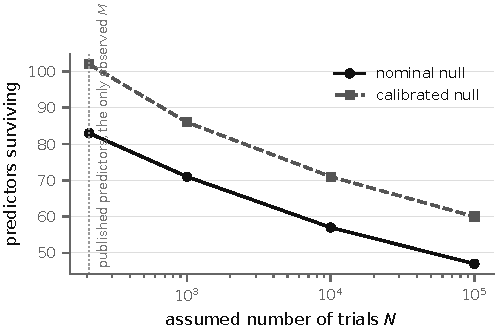
\includegraphics[width=0.62\linewidth]{figures/survival_vs_n}
\caption{Survival of the published predictors as a function of the assumed
number of tests, under the nominal and the calibrated null. The marked value is
the number of published predictors, the only $M$ that is observed.}
\label{fig:survival-vs-n}
\end{figure}


The dependence-aware procedures agree with the reading in
\S\ref{sec:thresholds}. On the common-sample panel the Reality Check gives
$p = \bzoorealityCheckP$ and the test for superior predictive ability
$p = \bzoospaP$, so the best of the published predictors comfortably beats zero
after accounting for the search over all of them; the \citet{romano2005}
step-down procedure rejects \bzooromanoWolfReject{} of the
\bzooromanoWolfN{} predictors with a common sample window. The median
\citet{harvey2015backtesting} haircut is \bzoohaircutMedianPct{} percent of the
reported Sharpe ratio.

\bibliographystyle{plainnat}
\bibliography{references}

\end{document}
